
%% bare_conf.tex
%% V1.3
%% 2007/01/11
%% by Michael Shell
%% See:
%% http://www.michaelshell.org/
%% for current contact information.
%%
%% This is a skeleton file demonstrating the use of IEEEtran.cls
%% (requires IEEEtran.cls version 1.7 or later) with an IEEE conference paper.
%%
%% Support sites:
%% http://www.michaelshell.org/tex/ieeetran/
%% http://www.ctan.org/tex-archive/macros/latex/contrib/IEEEtran/
%% and
%% http://www.ieee.org/

%%*************************************************************************
%% Legal Notice:
%% This code is offered as-is without any warranty either expressed or
%% implied; without even the implied warranty of MERCHANTABILITY or
%% FITNESS FOR A PARTICULAR PURPOSE!
%% User assumes all risk.
%% In no event shall IEEE or any contributor to this code be liable for
%% any damages or losses, including, but not limited to, incidental,
%% consequential, or any other damages, resulting from the use or misuse
%% of any information contained here.
%%
%% All comments are the opinions of their respective authors and are not
%% necessarily endorsed by the IEEE.
%%
%% This work is distributed under the LaTeX Project Public License (LPPL)
%% ( http://www.latex-project.org/ ) version 1.3, and may be freely used,
%% distributed and modified. A copy of the LPPL, version 1.3, is included
%% in the base LaTeX documentation of all distributions of LaTeX released
%% 2003/12/01 or later.
%% Retain all contribution notices and credits.
%% ** Modified files should be clearly indicated as such, including  **
%% ** renaming them and changing author support contact information. **
%%
%% File list of work: IEEEtran.cls, IEEEtran_HOWTO.pdf, bare_adv.tex,
%%                    bare_conf.tex, bare_jrnl.tex, bare_jrnl_compsoc.tex
%%*************************************************************************

% *** Authors should verify (and, if needed, correct) their LaTeX system  ***
% *** with the testflow diagnostic prior to trusting their LaTeX platform ***
% *** with production work. IEEE's font choices can trigger bugs that do  ***
% *** not appear when using other class files.                            ***
% The testflow support page is at:
% http://www.michaelshell.org/tex/testflow/



% Note that the a4paper option is mainly intended so that authors in
% countries using A4 can easily print to A4 and see how their papers will
% look in print - the typesetting of the document will not typically be
% affected with changes in paper size (but the bottom and side margins will).
% Use the testflow package mentioned above to verify correct handling of
% both paper sizes by the user's LaTeX system.
%
% Also note that the "draftcls" or "draftclsnofoot", not "draft", option
% should be used if it is desired that the figures are to be displayed in
% draft mode.
%
\documentclass[conference]{IEEEtran}
% Add the compsoc option for Computer Society conferences.
%
% If IEEEtran.cls has not been installed into the LaTeX system files,
% manually specify the path to it like:
% \documentclass[conference]{../sty/IEEEtran/}





% Some very useful LaTeX packages include:
% (uncomment the ones you want to load)


% *** MISC UTILITY PACKAGES ***
%
%\usepackage{ifpdf}
% Heiko Oberdiek's ifpdf.sty is very useful if you need conditional
% compilation based on whether the output is pdf or dvi.
% usage:
% \ifpdf
%   % pdf code
% \else
%   % dvi code
% \fi
% The latest version of ifpdf.sty can be obtained from:
% http://www.ctan.org/tex-archive/macros/latex/contrib/oberdiek/
% Also, note that IEEEtran.cls V1.7 and later provides a builtin
% \ifCLASSINFOpdf conditional that works the same way.
% When switching from latex to pdflatex and vice-versa, the compiler may
% have to be run twice to clear warning/error messages.






% *** CITATION PACKAGES ***
%
%\usepackage{cite}
% cite.sty was written by Donald Arseneau
% V1.6 and later of IEEEtran pre-defines the format of the cite.sty package
% \cite{} output to follow that of IEEE. Loading the cite package will
% result in citation numbers being automatically sorted and properly
% "compressed/ranged". e.g., [1], [9], [2], [7], [5], [6] without using
% cite.sty will become [1], [2], [5]--[7], [9] using cite.sty. cite.sty's
% \cite will automatically add leading space, if needed. Use cite.sty's
% noadjust option (cite.sty V3.8 and later) if you want to turn this off.
% cite.sty is already installed on most LaTeX systems. Be sure and use
% version 4.0 (2003-05-27) and later if using hyperref.sty. cite.sty does
% not currently provide for hyperlinked citations.
% The latest version can be obtained at:
% http://www.ctan.org/tex-archive/macros/latex/contrib/cite/
% The documentation is contained in the cite.sty file itself.






% *** GRAPHICS RELATED PACKAGES ***
%
\ifCLASSINFOpdf
  % \usepackage[pdftex]{graphicx}
  % declare the path(s) where your graphic files are
  % \graphicspath{{../pdf/}{../jpeg/}}
  % and their extensions so you won't have to specify these with
  % every instance of \includegraphics
  % \DeclareGraphicsExtensions{.pdf,.jpeg,.png}
\else
  % or other class option (dvipsone, dvipdf, if not using dvips). graphicx
  % will default to the driver specified in the system graphics.cfg if no
  % driver is specified.
  % \usepackage[dvips]{graphicx}
  % declare the path(s) where your graphic files are
  % \graphicspath{{../eps/}}
  % and their extensions so you won't have to specify these with
  % every instance of \includegraphics
  % \DeclareGraphicsExtensions{.eps}
\fi
% graphicx was written by David Carlisle and Sebastian Rahtz. It is
% required if you want graphics, photos, etc. graphicx.sty is already
% installed on most LaTeX systems. The latest version and documentation can
% be obtained at:
% http://www.ctan.org/tex-archive/macros/latex/required/graphics/
% Another good source of documentation is "Using Imported Graphics in
% LaTeX2e" by Keith Reckdahl which can be found as epslatex.ps or
% epslatex.pdf at: http://www.ctan.org/tex-archive/info/
%
% latex, and pdflatex in dvi mode, support graphics in encapsulated
% postscript (.eps) format. pdflatex in pdf mode supports graphics
% in .pdf, .jpeg, .png and .mps (metapost) formats. Users should ensure
% that all non-photo figures use a vector format (.eps, .pdf, .mps) and
% not a bitmapped formats (.jpeg, .png). IEEE frowns on bitmapped formats
% which can result in "jaggedy"/blurry rendering of lines and letters as
% well as large increases in file sizes.
%
% You can find documentation about the pdfTeX application at:
% http://www.tug.org/applications/pdftex





% *** MATH PACKAGES ***
%
%\usepackage[cmex10]{amsmath}
% A popular package from the American Mathematical Society that provides
% many useful and powerful commands for dealing with mathematics. If using
% it, be sure to load this package with the cmex10 option to ensure that
% only type 1 fonts will utilized at all point sizes. Without this option,
% it is possible that some math symbols, particularly those within
% footnotes, will be rendered in bitmap form which will result in a
% document that can not be IEEE Xplore compliant!
%
% Also, note that the amsmath package sets \interdisplaylinepenalty to 10000
% thus preventing page breaks from occurring within multiline equations. Use:
%\interdisplaylinepenalty=2500
% after loading amsmath to restore such page breaks as IEEEtran.cls normally
% does. amsmath.sty is already installed on most LaTeX systems. The latest
% version and documentation can be obtained at:
% http://www.ctan.org/tex-archive/macros/latex/required/amslatex/math/





% *** SPECIALIZED LIST PACKAGES ***
%
%\usepackage{algorithmic}
% algorithmic.sty was written by Peter Williams and Rogerio Brito.
% This package provides an algorithmic environment fo describing algorithms.
% You can use the algorithmic environment in-text or within a figure
% environment to provide for a floating algorithm. Do NOT use the algorithm
% floating environment provided by algorithm.sty (by the same authors) or
% algorithm2e.sty (by Christophe Fiorio) as IEEE does not use dedicated
% algorithm float types and packages that provide these will not provide
% correct IEEE style captions. The latest version and documentation of
% algorithmic.sty can be obtained at:
% http://www.ctan.org/tex-archive/macros/latex/contrib/algorithms/
% There is also a support site at:
% http://algorithms.berlios.de/index.html
% Also of interest may be the (relatively newer and more customizable)
% algorithmicx.sty package by Szasz Janos:
% http://www.ctan.org/tex-archive/macros/latex/contrib/algorithmicx/




% *** ALIGNMENT PACKAGES ***
%
%\usepackage{array}
% Frank Mittelbach's and David Carlisle's array.sty patches and improves
% the standard LaTeX2e array and tabular environments to provide better
% appearance and additional user controls. As the default LaTeX2e table
% generation code is lacking to the point of almost being broken with
% respect to the quality of the end results, all users are strongly
% advised to use an enhanced (at the very least that provided by array.sty)
% set of table tools. array.sty is already installed on most systems. The
% latest version and documentation can be obtained at:
% http://www.ctan.org/tex-archive/macros/latex/required/tools/


%\usepackage{mdwmath}
%\usepackage{mdwtab}
% Also highly recommended is Mark Wooding's extremely powerful MDW tools,
% especially mdwmath.sty and mdwtab.sty which are used to format equations
% and tables, respectively. The MDWtools set is already installed on most
% LaTeX systems. The lastest version and documentation is available at:
% http://www.ctan.org/tex-archive/macros/latex/contrib/mdwtools/


% IEEEtran contains the IEEEeqnarray family of commands that can be used to
% generate multiline equations as well as matrices, tables, etc., of high
% quality.


%\usepackage{eqparbox}
% Also of notable interest is Scott Pakin's eqparbox package for creating
% (automatically sized) equal width boxes - aka "natural width parboxes".
% Available at:
% http://www.ctan.org/tex-archive/macros/latex/contrib/eqparbox/





% *** SUBFIGURE PACKAGES ***
%\usepackage[tight,footnotesize]{subfigure}
% subfigure.sty was written by Steven Douglas Cochran. This package makes it
% easy to put subfigures in your figures. e.g., "Figure 1a and 1b". For IEEE
% work, it is a good idea to load it with the tight package option to reduce
% the amount of white space around the subfigures. subfigure.sty is already
% installed on most LaTeX systems. The latest version and documentation can
% be obtained at:
% http://www.ctan.org/tex-archive/obsolete/macros/latex/contrib/subfigure/
% subfigure.sty has been superceeded by subfig.sty.



%\usepackage[caption=false]{caption}
%\usepackage[font=footnotesize]{subfig}
% subfig.sty, also written by Steven Douglas Cochran, is the modern
% replacement for subfigure.sty. However, subfig.sty requires and
% automatically loads Axel Sommerfeldt's caption.sty which will override
% IEEEtran.cls handling of captions and this will result in nonIEEE style
% figure/table captions. To prevent this problem, be sure and preload
% caption.sty with its "caption=false" package option. This is will preserve
% IEEEtran.cls handing of captions. Version 1.3 (2005/06/28) and later
% (recommended due to many improvements over 1.2) of subfig.sty supports
% the caption=false option directly:
%\usepackage[caption=false,font=footnotesize]{subfig}
%
% The latest version and documentation can be obtained at:
% http://www.ctan.org/tex-archive/macros/latex/contrib/subfig/
% The latest version and documentation of caption.sty can be obtained at:
% http://www.ctan.org/tex-archive/macros/latex/contrib/caption/




% *** FLOAT PACKAGES ***
%
%\usepackage{fixltx2e}
% fixltx2e, the successor to the earlier fix2col.sty, was written by
% Frank Mittelbach and David Carlisle. This package corrects a few problems
% in the LaTeX2e kernel, the most notable of which is that in current
% LaTeX2e releases, the ordering of single and double column floats is not
% guaranteed to be preserved. Thus, an unpatched LaTeX2e can allow a
% single column figure to be placed prior to an earlier double column
% figure. The latest version and documentation can be found at:
% http://www.ctan.org/tex-archive/macros/latex/base/



%\usepackage{stfloats}
% stfloats.sty was written by Sigitas Tolusis. This package gives LaTeX2e
% the ability to do double column floats at the bottom of the page as well
% as the top. (e.g., "\begin{figure*}[!b]" is not normally possible in
% LaTeX2e). It also provides a command:
%\fnbelowfloat
% to enable the placement of footnotes below bottom floats (the standard
% LaTeX2e kernel puts them above bottom floats). This is an invasive package
% which rewrites many portions of the LaTeX2e float routines. It may not work
% with other packages that modify the LaTeX2e float routines. The latest
% version and documentation can be obtained at:
% http://www.ctan.org/tex-archive/macros/latex/contrib/sttools/
% Documentation is contained in the stfloats.sty comments as well as in the
% presfull.pdf file. Do not use the stfloats baselinefloat ability as IEEE
% does not allow \baselineskip to stretch. Authors submitting work to the
% IEEE should note that IEEE rarely uses double column equations and
% that authors should try to avoid such use. Do not be tempted to use the
% cuted.sty or midfloat.sty packages (also by Sigitas Tolusis) as IEEE does
% not format its papers in such ways.





% *** PDF, URL AND HYPERLINK PACKAGES ***
%
%\usepackage{url}
% url.sty was written by Donald Arseneau. It provides better support for
% handling and breaking URLs. url.sty is already installed on most LaTeX
% systems. The latest version can be obtained at:
% http://www.ctan.org/tex-archive/macros/latex/contrib/misc/
% Read the url.sty source comments for usage information. Basically,
% \url{my_url_here}.





% *** Do not adjust lengths that control margins, column widths, etc. ***
% *** Do not use packages that alter fonts (such as pslatex).         ***
% There should be no need to do such things with IEEEtran.cls V1.6 and later.
% (Unless specifically asked to do so by the journal or conference you plan
% to submit to, of course. )


% correct bad hyphenation here
\hyphenation{op-tical net-works semi-conduc-tor}

%\documentclass[11pt,oneside,a4paper]{article}
\usepackage{amsmath}
\usepackage{cases}
%\usepackage[top=1in, bottom=1in, left=1.25in, right=1.25in]{geometry}
\usepackage{stmaryrd}

\usepackage{pgf}
\usepackage{tikz}
\usepackage{amssymb}
\usepackage{amsthm}
\usepackage{framed,multicol}
\usepackage{enumerate}
\usepackage{makecell}
\usepackage{listings}
\usepackage{cite}

%\usepackage{amsmath}

\usetikzlibrary{arrows,automata}

\newtheorem{mydef}{Definition}[section]
\newtheorem{mytheo}{Theorem}[section]
\newtheorem{lemma}{Lemma}[section]
\newtheorem{prop}{Property}[section]
\newtheorem{cor}{Corollary}[section]

\renewcommand{\labelenumi}{\arabic{enumi}. }
\renewcommand{\labelenumii}{\labelenumi\alph{enumii}) }
\renewcommand{\labelenumiii}{\labelenumii\roman{enumiii}: }

\newcommand{\rNum}[1]{\expandafter{\romannumeral #1\relax}}
\newcommand{\rNUM}[1]{\uppercase\expandafter{\romannumeral #1\relax}}

\newcommand{\xian}{\noindent\rule{88mm}{0.2pt}}

\newcommand{\fred}[0]{\color{red}}
\newcommand{\bff}[1]{\mathbf{#1}}
\newcommand{\mbb}[1]{\mathbb{#1}}
\newcommand{\mcl}[1]{\mathcal{#1}}
\newcommand{\spc}[1]{\begin{spacing}{#1}}
\newcommand{\spce}{\end{spacing}}

\newcommand{\quan}[1]{\textcircled{\small{#1}}}

\IEEEoverridecommandlockouts

\begin{document}
%
% paper title
% can use linebreaks \\ within to get better formatting as desired
%\title{An Approach of Verification of STeC }
%\title{Transformation of Spatial-Temporal Consistence Language to Timed Automata}
\title{A Verification Framework of Spatio-Temporal Consistent Language STeC based on Timed Automata}

% author names and affiliations
% use a multiple column layout for up to three different
% affiliations
\author{\IEEEauthorblockN{Yuanrui Zhang}
\IEEEauthorblockA{Institute of Software Engineering,\\
East China Normal University,\\
Shanghai, China\\
Polytech Nice Sophia,\\
University Nice Sophia Antipolis,\\
Nice, France\\
Email: yuanrui1990.zhang@gmail.com}
\and
\IEEEauthorblockN{Frederic Mallet}
\IEEEauthorblockA{ Univ. Nice Sophia Antipolis, \\
CNRS, I3S, UMR 7271, \\
06900 Sophia Antipolis, France \\
(NOTE: Member of Aoste team (INRIA/I3S)\\
Email: Frederic.Mallet@unice.fr\\
}
\and
\IEEEauthorblockN{Yixiang Chen}
\IEEEauthorblockA{MoE Engineering Research Center for\\
Software/Hardware Co-design \\
Technology and Application,\\
East China Normal University, \\
Shanghai, China\\
Email: yxchen@sei.ecnu.edu.cn}
\IEEEcompsocitemizethanks{\IEEEcompsocthanksitem
* \small  Yixiang Chen: The Communication author}
}

% conference papers do not typically use \thanks and this command
% is locked out in conference mode. If really needed, such as for
% the acknowledgment of grants, issue a \IEEEoverridecommandlockouts
% after \documentclass

% for over three affiliations, or if they all won't fit within the width
% of the page, use this alternative format:
%
%\author{\IEEEauthorblockN{Michael Shell\IEEEauthorrefmark{1},
%Homer Simpson\IEEEauthorrefmark{2},
%James Kirk\IEEEauthorrefmark{3},
%Montgomery Scott\IEEEauthorrefmark{3} and
%Eldon Tyrell\IEEEauthorrefmark{4}}
%\IEEEauthorblockA{\IEEEauthorrefmark{1}School of Electrical and Computer Engineering\\
%Georgia Institute of Technology,
%Atlanta, Georgia 30332--0250\\ Email: see http://www.michaelshell.org/contact.html}
%\IEEEauthorblockA{\IEEEauthorrefmark{2}Twentieth Century Fox, Springfield, USA\\
%Email: homer@thesimpsons.com}
%\IEEEauthorblockA{\IEEEauthorrefmark{3}Starfleet Academy, San Francisco, California 96678-2391\\
%Telephone: (800) 555--1212, Fax: (888) 555--1212}
%\IEEEauthorblockA{\IEEEauthorrefmark{4}Tyrell Inc., 123 Replicant Street, Los Angeles, California 90210--4321}}




% use for special paper notices
%\IEEEspecialpapernotice{(Invited Paper)}




% make the title area
\maketitle


\begin{abstract}
%\boldmath
Intelligent Transportation Systems (ITS) are a class of quickly evolving modern safety-critical embedded systems. Dealing with their growing complexity demands a high-level formal modeling language along with adequate verification techniques. STeC has recently been introduced as a process algebra that deals natively with both spatial and temporal properties. Even though STeC has a good abstraction and enough expressive power for modeling ITS in high-level. It does not provide a direct support for verification both in theory and application. We propose to encode STeC models as Timed Automata (abbreviated as TA) and introduce CCSL as its specification language on its abstract level to provide such a support. We illustrate our verification strategy on a simple ITS example.
\end{abstract}
% IEEEtran.cls defaults to using nonbold math in the Abstract.
% This preserves the distinction between vectors and scalars. However,
% if the conference you are submitting to favors bold math in the abstract,
% then you can use LaTeX's standard command \boldmath at the very start
% of the abstract to achieve this. Many IEEE journals/conferences frown on
% math in the abstract anyway.

% no keywords




% For peer review papers, you can put extra information on the cover
% page as needed:
% \ifCLASSOPTIONpeerreview
% \begin{center} \bfseries EDICS Category: 3-BBND \end{center}
% \fi
%
% For peerreview papers, this IEEEtran command inserts a page break and
% creates the second title. It will be ignored for other modes.
\IEEEpeerreviewmaketitle



\section{Introduction}
% no \IEEEPARstart
\ifx
Our reliance on the functioning of embedded real-time systems is growing rapidly. And formal methods
play an important role for improving the safety and security of embedded real-time systems.
\fi

Intelligent Transportation Systems (ITS) are a class of time-sensitive and safety-critical systems. Dealing with their safety issues and their growing complexity on both architecture and communication aspects demands high-level though formal specification models, adequate verification languages along with adequate verification tools. In history, many formal methods have been developed over the last two decades. They are classified according to two categories: untimed and timed formal methods. The former includes many early works in the area of process algebra, automata theory and classic model checking theory. The latter mainly are the timed versions of different classes of formal languages.

In the field of process algebra, CSP (\cite{hoare78}, \cite{schneider06}) was firstly proposed by Hoare in 1978 as the first process algebra modeling the communication behaviour in concurrent systems. $\pi$-calculus~\cite{milner82}, simular to $\lambda$-calculus, is a rewriting languages describing and analyzing properties of concurrent computations. Later,   Timed-CSP~\cite{schneider95} was proposed in 1995 as a timed version of CSP where a new operator 'WAIT' is added.

 In automata theory, Robin and Scott initially proposed the concept of finite automata in 1959. Timed Automata (TA)~\cite{alur94} was introduced by Alur and Dill in 1994.

\ifx
 \xian
* {\small  Yixiang Chen: The Communication author}
\fi

 It has inspired a lot of works as they introduced real-valued clocks thus making 'time' a first-class citizen of the specification languages. Hybrid automata was proposed in 1996 by Henzinger.

 LTL (Linear Temporal Language) and CTL (Computational Tree Language) are prominent specification languages proposed in the field of model checking. TCTL was proposed as the timed version of CTL which is used in the verification of Timed Automata.
 In 2005, the IEEE PSL (Property Specification Language) was proposed.

 While in untimed formal models, only the description of functionality of behaviours of system is stressed, in timed formal models, the real-time performance of behaviours is stressed. Each behaviour is required to be fired at the right time, time correctness becomes as important as functional correctness. However, for some classes of systems (especially Intelligent Transportation Systems), behaviours are usually required to be fired not only at the right time but also the right location. So they are not only time-sensitive but spatio-time sensitive. For example, in a 'Railroad Crossing System' (see Fig.~\ref{RCP}) that will be introduced later, a train is always required to receive a message from gate at the right location and time (more examples are available in \cite{chen12}). We believe that such types of systems demand a new formal modeling language that stresses the spatio-temporal consistence of behaviours of systems in its semantics. For this purpose, STeC~\cite{chen12} (Spatio-Temporal Consistence Language) was proposed as a process algebra to build spatio-temporal models.

 As computer systems are growing on size and complexity, high-level specification engineering models are becoming more and more important and are widely used through industry, like AADL, SysML and UML (the Unified Modeling Language). Such models should have a proper
formal semantics if verification is intended. CCSL~\cite{andre08} (The Clock Constraint Specification Language) was initially proposed as a companion language of UML profile for MARTE, but later had been developed as an independent formal specification language. CCSL provides formal semantics support for UML models, with its abstract clock models and progressive refinement.
In CCSL, logic clock is understood as a sequence of occurences, and the logical, both causal and temporal, relationships between behaviours is described as 'CCSL constraints' that restrict the way the logical clock can tick, i.e., the instants at which the events may occur. Logical clocks are not only good for modeling sequences of occurring events, but also sequences of properly ordered locations (like tracks in ITS). This is this particular property that we further study here.

Formal verification is used in proving the correctness of highly-critical systems with respect to a certain formal specification (or property). Over the past years, many verification techniques have been proposed and developed, along with verification tools.
UPPAAL is one of widely accepted verification tools based on Timed Automata theory.

Rigorously speaking, CCSL is not equivalent to pure Timed Automata. In \cite{gascon11}, the comparison between CCSL and PSL is analyzed. \cite{mallet13} gives a state-base representation for CCSL. \cite{suryadevara13} gives an encoding from part of CCSL (called safety CCSL) into Timed Automata. Later we explain why such an encoding is essential for verification purpose.

In this paper, we propose a new verification framework where we use STeC as a formal system-modeling language, and CCSL for the specification of properties of system. We introduce CCSL as a specification language in the domain of STeC. Then we focus on the encoding from STeC into TA, with it we apply UPPAAL as a verification tool on TA to verify properties.

Section 2 gives the academic background that are essential for introducing the contributions of this paper. In Section 3 we propose a verification framework of STeC and CCSL. In Section 4, we introduce STeC traces and introduce CCSL as a specification language in the domain of STeC. In Section 5, we focus on the translation from STeC into Timed Automata for verification purpose. In Section 6, we use a simple example of Intelligent Transportation Systems to illustrate models and verification techniques under the new verification framework. Section 7 summarizes the results.

\section{Academic Background}
In this section, some basic definitions about STeC, CCSL and TA are introduced. These definitions are necessary for understanding the contribution part. For the original definitions and more details, see \cite{alur94}, \cite{chen12}, \cite{andre09}, \cite{CK05} and \cite{abdulla10}.

\subsection{Introduction of STeC}
Yixiang Chen introduced the Spatio-Temporal Consistence Language in 2010~\cite{chen12} and set up its formal semantics with his colleagues in \cite{wu13}. Unlike the traditional formal modeling languages, it stresses the location and the time of an event of spatio-time sensitive systems, especially ITS. An event (or action) is fired at a given location and a given time.
For example, in a Train Scheduling System (see \cite{chen12}, \cite{wu13}), trains travel from one platform to another with very strict time restrictions. Fig.~\ref{g147} shows a scheduling table of train 'G147', where we see that train 'G147' departs from 'Beijing' at 14:36, runs for 131km and arrives at 'Tianjin' at 15:10, stops for 2 minutes and departs at 15:12,.... If a train does not arrive at station at the expected time, then collisions might happen.
This characteristic of STeC makes it a powerful and convenient formal modeling language for ITS (for more examples, see \cite{chen12}, \cite{wu13}).
However, STeC does not provide at the moment any support for formal verification.

\begin{figure}
     \centering
\includegraphics[width=10cm]{graph/g147.PNG}
\caption{Scheduling Table of Train 'G147'}
\label{g147}
\end{figure}

\subsubsection{Syntax of STeC}
Like other process algebras, in STeC we use 'action' to describe behaviours (or events) of a system, as a set of communicating agents. An 'action' in STeC consists of an action name (also called 'alphabet'), a start location, a start time point, a duration of time and a end location (if an action depends on the position of the Agent). For example, let us consider the following statement:

 \begin{center}'the train "$G$" approaches at location "Lapp" at time $t$ during $\delta$ time units'\end{center}

 where '$G$' is the name of train, 'Lapp' is a location, $t$ is a time and $\delta$ is a duration. It is stated in STeC like this: $$Approach^G_{(Lapp,t)}(\delta)$$

 where 'Approach' is an action name (or alphabet), the action 'Approach' is fired at location 'Lapp' and time $t$, and lasts $\delta$ units.

Consider now a second example a bit more complex:

\begin{center}
'After receiving Message "Cross" at location "Lpass" and at
time $t$, the train passes the crossroad in $d$ units of time'
\end{center}

This is stated in STeC as follows:
$$\bff{Get}_{(Lpass,t)}(Cross) ; Pass_{(Lpass,t)}(d)$$

\begin{center}(Note: the name of agent '$G$' is always omitted.)\end{center}

Action $\bff{Get}$ is call a 'communication' action, and is aimed at communicating with other agents. ';' is a binary operator called 'sequence', meaning that action $\bff{Get}$ is fired, then action $Pass$ is fired. The composition of actions is an action in STeC. There are many other binary operators in STeC.

Informally, in STeC we call an action 'atomic' if it can not be divided into several 'smaller' actions. In the example above, $\bff{Get}$ and $Pass$ are atomic actions, the composition of them are not atomic.

The formal definition of syntax of STeC is given below in Backus-Naur Form:

$$A\ ::=\ \mathbf{Send}^{G \rightharpoonup G^\prime}_{(l,t)}(m)\ |\ \mathbf{Get}^{G \leftharpoonup G^\prime}_{(l,t)}(m)$$
$$B\ ::=\ \alpha_{(l,t)}(l^\prime,\delta)\ |\ \beta_{(l,t)}(\delta)$$
$$P\ ::\ =\ \mathbf{Stop}^{G}_{(l,t)}\ |\ \mathbf{Skip}^{G}_{(l,t)}\ |\ A\ |\ B\ |\ $$
$$P;P\ |\ P \parallel P\ |\ []_{i \in I}B_i \to P_i\ |\ P \unrhd_{\delta} P\ |$$
$$B\to P\ |\ P \unrhd ([]_{i \in I}A_i \to P_i)$$

In STeC, there are two types of atomic actions: type $A$ and type $B$. Type $A$ is for communication purpose.
$\mathbf{Send}^{G \rightharpoonup G^\prime}_{(l,t)}(m)$ means that agent $G$ sends a message $m$ to agent $G^\prime$.
$\mathbf{Get}^{G \leftharpoonup G^\prime}_{(l,t)}(m)$ means that agent $G$ receives a message $m$ from agent $G^\prime$.
Type $B$ are other actions, $\alpha$ and $\beta$ are to be replaced by user-defined action names (like $Pass$ or $Approach$ in the previous examples). Action $\alpha^{G}_{(l,t)}(l^{\prime},\delta)$
means that the action of agent $G$ is fired at location $l$ and time $t$, after $\delta$ time, agent $G$ jumps to $l^\prime$ from $l$. While $\beta^{G}_{(l,t)}(\delta)$ stays in location $l$ after the execution.

 $\mathbf{Stop}^{G}_{(l,t)}$, $\mathbf{Skip}^{G}_{(l,t)}$ are special atomic processes.

'$;$' is the sequence operator, $P;Q$ means that process $P$ is fired then process $Q$ is fired.

'$\parallel$' is the parallel operator, $P \parallel Q$ means that process $P$ and $Q$ are fired concurrently.
While $[]_{i \in I}B_i \to P_i$ is a guard choice, meaning that if $B_i$ holds for some $i$, then $P_i$ is fired. If several $B_i$ holds at the same time, the choice of $P_i$ is a nondeterministic choice.


'$\unrhd$' is the 'interrupt' operator. $P \unrhd_{\delta} Q$ behaves as $P$ for up to $\delta$ time units and then is interrupted by $Q$.
$P \unrhd ([]_{i \in I}A_i \to P_i)$ initially
fires P and is interrupted on occurrence of the atomic command $A_i$ and then proceeds like $P_i$.
Here $A_i$ is an action of type $A$. If several $A_i$ are fired simultaneously, the choice '$[]$' here is a nondeterministic choice.

For more details about the syntax of 	STeC, refer to \cite{chen12} and \cite{wu13}.

\subsubsection{The Operational Semantics of STeC} A storage $\sigma$ is introduced in STeC as the storage of messages between agents. Let
$\sigma \subseteq \mathbb{M}$, $\mathbb{M}$ is the set of messages of the form $m_{G \rightharpoonup G^\prime}$. Here we
use $\mathbf{Sto}$ to represent the set of storages and it is easy to see that:\ $\mathbf{Sto}\ \subseteq \ 2^{\mathbb{M}}$.

Let $\mathbf{Loc}$ be the set of locations. $\mathbb{R}^+$ is the non-negative real set. An environment is a triple $(a,u,\sigma)$ where $\sigma$ is a storage, $a$ is a location and $u$ is time. We use the notation $\mathcal{E}$ to represent the set of all the environments: $\mathcal{E}\ =\ \mathbf{Loc} \times \mathbb{R}^+ \times \mathbf{Sto} $.

%Let $\mathbb{B}=\{B | B\ is\ a\ 'B'\ type\ formula\ in\ STeC\}$(see the syntax in STeC). A function $\mathcal{T}: %\mathbb{B} \to \{0,1\}$ is defined as the truth valuation function. We have $\mathcal{T}(B)=1$ (resp. %$\mathcal{T}(B)=0$) if $B$ is true (resp. false).

Let $\mathbb{B}=\{B\ |\ B$ is action type 'B' in STeC $\}$ (see the syntax of STeC). A function $\mathcal{T}: \mathbb{B} \to \{0,1\}$ is defined as the truth valuation function. We have $\mathcal{T}(B)=1$ (resp. $\mathcal{T}(B)=0$) if $B$ is true (resp. false).

A configuration of process $P$ is defined as a tuple $\langle P,(a,u,\sigma) \rangle$. Define $\mathbf{Stconf}=\{\langle P,(a,u,\sigma) \rangle\ |\ P$ is a process and for some $a, u,\sigma\}$
as the set of all configurations in STeC.

The transition relation of STeC $\hookrightarrow_{STeC}$ is a function:
$$
\hookrightarrow_{STeC}: \mathbf{Stconf} \to 2^{\mathbf{Stconf}}
$$
 Any transition relation is denoted as $\langle P,(a,u,\sigma) \rangle \to \langle P^\prime,(a^\prime,u^\prime,\sigma^\prime) \rangle$ iff (if and only if) $\hookrightarrow_{STeC}(\langle P,(a,u,\sigma) \rangle)=
\langle P^\prime,(a^\prime,u^\prime,\sigma^\prime) \rangle$ holds.

$\tau$ is a function that maps each process in STeC to the non-negative real set $\mathbb{R}^+$. It computes the duration time for each process. For example, $\tau(\alpha_{(l,t)}(l^\prime,\delta))=\delta$. For more details, see \cite{chen12}.

The operational semantics of STeC is listed as follows. For more details, refer to \cite{chen12}.

\begin{framed}
    \begin{itemize}
    \setlength{\itemsep}{0.05in}
    \item
     $\frac{a=l,u=t}{\langle \mathbf{Send}^{G \rightharpoonup G^\prime}_{(l,t)}(m),(a,u,\sigma) \rangle \to
     \langle E,(l,t,\sigma \cup \{m_{G\rightharpoonup G^\prime}\}) \rangle}$
     \item
     $\frac{a=l,u=t}{\langle \mathbf{Get}^{G \leftharpoonup G^\prime}_{(l,t)}(m),(a,u,\sigma) \rangle \to
     \langle E,(l,t,\sigma \backslash \{m_{G\leftharpoonup G^\prime}\}) \rangle}$
     \item
     $\frac{a=l,u=t}{\langle \alpha_{(l,t)}(l^\prime,\delta),(a,u,\sigma) \rangle \to
     \langle E,(l^\prime,t+\delta,\sigma) \rangle}$
     \item
      $\frac{a=l,u=t}{\langle \beta_{(l,t)}(\delta),(a,u,\sigma) \rangle \to
     \langle E,(l,t+\delta,\sigma) \rangle}$
     \item
     $\frac{a=l,u=t}{\langle \mathbf{Stop}^{G}_{(l,t)},(a,u,\sigma) \rangle \to
     \langle E,(l,t+1,\sigma) \rangle}$
     \item
     $\frac{a=l,u=t}{\langle \mathbf{Skip}^{G}_{(l,t)},(a,u,\sigma) \rangle \to
     \langle E ,(l,t,\sigma) \rangle}$
     \item
     $\frac{\langle P,(a,u,\sigma) \rangle \to \langle P^\prime,(a^\prime,u^\prime,\sigma^\prime) \rangle}
     {\langle P;Q,(a,u,\sigma) \rangle \to  \langle P^\prime;Q,(a^\prime,u^\prime,\sigma^\prime) \rangle}$

     \ifx
     \item
     $\frac{\langle P,(a,u,\sigma) \rangle \to \langle P^\prime,(a_{1},u_{1},\sigma_1) \rangle,\ \langle Q,(a,u,\sigma) \rangle \to \langle Q^\prime,(a_2,u_2,\sigma_2) \rangle}
     {\langle P[]Q,(a,u,\sigma) \rangle \to \{\langle P^\prime,(a_1,u_1,\sigma_1) \rangle, \langle Q^\prime,(a_2,u_2,\sigma_2) \rangle \} }$
     \fi

     \item
     $\frac{\langle P,(a,u,\sigma) \rangle \to \langle P^\prime,(a^\prime,u^\prime,\sigma_1) \rangle}
     {\langle P \parallel Q,(a,u,\sigma) \rangle \to \langle P^\prime \parallel Q,(a^\prime,u^\prime,\sigma_1) \rangle}$
     \item
     $\frac{\langle Q,(a,u,\sigma) \rangle \to \langle Q^\prime,(a^\prime,u^\prime,\sigma_2) \rangle}
     {\langle P \parallel Q,(a,u,\sigma) \rangle \to \langle P^\prime \parallel Q^\prime,(a^\prime,u^\prime,\sigma_2) \rangle}$
     \item
      $\frac{\langle P,(a,u,\sigma) \rangle \to \langle P^\prime,(a_1,u_1,\sigma_1) \rangle,\ \langle Q,(a,u,\sigma) \rangle \to \langle Q^\prime,(a_2,u_2,\sigma_2) \rangle}
     {\langle P \parallel Q,(a,u,\sigma) \rangle \to \langle P^\prime \parallel Q^\prime,(a^\prime,u^\prime,\sigma_1 \uplus \sigma_2) \rangle}$
     \item
     $\frac{\mathcal{T}(B_i)=1\ for\ i\in I,\ \langle B_i,(a,u,\sigma)\rangle\to\langle E,(a_i,u_i,\sigma_i)\rangle}{\langle []_{i \in I}B_i \to P_i,(a,u,\sigma) \rangle \to \bigcup_{i\in I}\{\langle P_i,(a_i,u_i,\sigma_i) \rangle\}}$

     \item
     $\frac{\langle P,(a,u,\sigma) \rangle \to \langle P^\prime,(a^\prime,u^\prime,\sigma^\prime) \rangle \  \wedge \ u^\prime \leq \delta}{\langle P \unrhd_{\delta} Q,(a,u,\sigma) \rangle \to \langle P^\prime \unrhd_{\delta} Q,(a^\prime,u^\prime,\sigma^\prime) \rangle}$
     \item
     $\frac{\langle P,(a,u,\sigma) \rangle \to \langle P^\prime,(a^\prime,u^\prime,\sigma^\prime) \rangle \  \wedge \ u^\prime > \delta}{\langle P \unrhd_{\delta} Q,(a,u,\sigma) \rangle \to \langle Q,(a^{\prime\prime},\delta,\sigma^{\prime\prime}) \rangle}$
     \item
     $\frac{\mathcal{T}(B)=1,\ \langle B,(a,u,\sigma)\rangle\to\langle E,(a^\prime,u^\prime,\sigma^\prime\rangle}{\langle B \to P,(a,u,\sigma) \rangle \to \langle P,(a^\prime,u^\prime,\sigma^\prime) \rangle}$
     \item
     $\frac{\mathcal{T}(B)=0,\ \langle B,(a,u,\sigma)\rangle\to\langle E,(a^\prime,u^\prime,\sigma^\prime\rangle}{\langle B \to P,(a,u,\sigma) \rangle \to \langle \mathbf{Stop}^{G}_{(l,t)},(a^\prime,u^\prime,\sigma^\prime) \rangle}$

     \item
     $\frac{\langle A_i,(a,u,\sigma)\rangle \to \langle E,(a^\prime,u^\prime,\sigma^\prime)\rangle,\ for\ i\in I}
     {\langle P \unrhd ([]_{i \in I}A_i \to P_i),(a,u,\sigma)\rangle \to \bigcup_{i\in I}\{\langle P_i,(a^\prime,u^\prime,\sigma^\prime)\rangle\}}
     $
    \end{itemize}
\end{framed}

\subsection{Introduction of CCSL}
The Clock Constraint Specification Language (CCSL) was initially proposed by Charles Andre and Frederic Mallet in 2008~\cite{andre08}. It has then evolved as a fully-fledged specification language to augment engineering models (UML amongst others) with a formal causal and timed semantics (see \cite{mallet10}). The rest of this section focuses on basic concepts. For more details, see the relative references.

\subsubsection{Clock}
In CCSL, a clock is a ordered sequence of events (or behaviours). The logical relationships between clocks are binary operators between clocks. Here is an example:

\begin{center}'event $a$ is always fired before event $b$'\end{center}

which is denoted as $c_a\prec c_b$ in CCSL. Fig.~\ref{aprecb} shows an equivalent (infinite) automata of it, which contains an error state. In Fig.~\ref{aprecb}, the only possible way of getting to the error state is to have a scenario where at a given instant, $b$ has occurred more often than $a$.

\begin{figure}[htp]
\centering
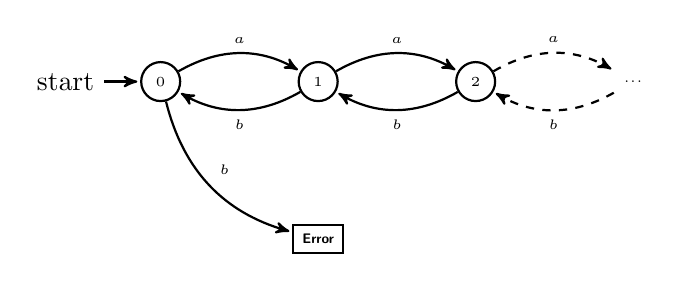
\begin{tikzpicture}[->,>=stealth',shorten >=1pt,auto,node distance=2cm,
  thick,main node/.style={circle,fill=white,draw,font=\sffamily\tiny\bfseries},
  sub node/.style={circle,fill=white,draw,font=\sffamily\tiny\bfseries},
  red node/.style={circle,fill=white,draw,font=\sffamily\tiny\bfseries},
  rec node/.style={rectangle,fill=white,draw,font=\sffamily\tiny\bfseries}]

  \node[initial,main node] (1) [] {$0$};
  \node[main node] (2) [right of=1] {$1$};
  \node[main node] (3) [right of=2]{$2$};
  \node[rec node,draw=none] (4) [right of=3]{$...$};
  \node[rec node] (5) [below of=2]{Error};

 	\path[every node/.style={font=\sffamily\tiny},dashed]
    (3) edge [bend left] node {$a$} (4)
    (4) edge [bend left] node {$b$} (3)
    ;

    \path[every node/.style={font=\sffamily\tiny}]
    (1) edge [bend left] node {$a$} (2)
    (2) edge [bend left] node {$a$} (3)
    (3) edge [bend left] node {$b$} (2)
    (2) edge [bend left] node {$b$} (1)
    (1) edge [bend right] node {$b$} (5)
    ;

\end{tikzpicture}
\caption{The automata(infinite) of $c_a\prec c_b$}
\label{aprecb}
\end{figure}

\begin{figure}[htp]
\centering
\includegraphics[width=3in]{graph/prec.png}
\caption{A possible trace of $c_a\prec c_b$}
\label{precclock}
\end{figure}

Fig.\ref{precclock} shows a possible trace of $c_a\prec c_b$ that is generated by Timesquare~\cite{deantoni12}---an analysis framework dedicated to CCSL.
%easily see that event $a$ is always fired before event $b$.

Another example is the concept of 'subclock' in CCSL:

\begin{center}'event $a$ occurs implies event $b$ occurs'\end{center}

It means that whenever $a$ is fired, $b$ is fired simultaneously. Fig.\ref{asubsetb} shows the automata (this time it is finite) of $c_a\subseteq c_b$. From Fig.~\ref{asubsetb}, it is clear to see that event $a$ is never fired alone since $c_a$ is a subclock of $c_b$. Fig.~\ref{subclock} shows a possible trace.

\begin{figure}[htp]
\centering
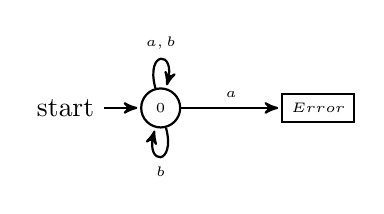
\begin{tikzpicture}[->,>=stealth',shorten >=1pt,auto,node distance=2cm,
  thick,main node/.style={circle,fill=white,draw,font=\sffamily\tiny\bfseries},
  sub node/.style={circle,fill=white,draw,font=\sffamily\tiny\bfseries},
  red node/.style={circle,fill=white,draw,font=\sffamily\tiny\bfseries},
  rec node/.style={rectangle,fill=white,draw,font=\sffamily\tiny\bfseries}]

  \node[initial,main node] (1) [] {$0$};
  \node[rec node] (2) [right of=1] {$Error$};

 	\path[every node/.style={font=\sffamily\tiny},dashed]
    ;

    \path[every node/.style={font=\sffamily\tiny}]
    (1) edge [loop above] node {$a,b$} (1)
    (1) edge [loop below] node {$b$} (1)
    (1) edge node {$a$} (2)
    ;

\end{tikzpicture}
\caption{The automata of $c_a\subseteq c_b$}
\label{asubsetb}
\end{figure}

\begin{figure}[htp]
\centering
\includegraphics[width=3in]{graph/subclock2.png}
\caption{A possible trace of $c_a\subseteq c_b$}
\label{subclock}
\end{figure}

Formally, a Clock in CCSL is a tuple $\langle \mathcal{I}, \prec, \mathcal{D}, \lambda, \mu \rangle$, where $\mathcal{I}$ is a set
of instants(possibly infinite), $\prec$ is a quasi-order relation on $\mathcal{I}$, $\mathcal{D}$ is a set of labels, $\lambda\ :\ \mathcal{I} \to \mathcal{D}$ is a labelling function, $\mu$ is a symbol,
standing for a 'unit' of time.

A discrete-time clock in CCSL is a clock with a descrete set of instants $\mathcal{I}$. Since $\mathcal{I}$ is discrete,
it can be indexed by natural numbers in a way that respects the ordering on $\mathcal{I}$: set $\mathbb{N}^{+} = \mathbb{N} \backslash \{0\}$, $idx\ :\ \mathcal{I} \to \mathbb{N}^{+}$, $\forall i \in \mathcal{I}, idx(i) = k$ if and only if $i$ is the $k^{th}$ instant in $\mathcal{I}$.

Let $c=\langle \mathcal{I}, \prec, \mathcal{D}, \lambda, \mu \rangle$ be a CCSL clock. $c[k]$ denotes the $k^{th}$ element in $\mathcal{I}$, then we have $k=idx(c[k])$.
Let $\lambda_i=\lambda(c[i])$.

\subsubsection{Clock Constraint}
In CCSL, we use 'clock' to denote the occurrence of events in a system, binary operations between clocks describe the logical relationship between clocks. They are divided into two basic type of operations, one is called 'Sub Clock' and the other is 'Precedence'. All binary operators in CCSL are derived from these two type of basic operations. For example, binary operations like 'Equality', 'Restriction', 'Discretization', 'Filtering' are derived from 'Sub Clock'. And operations such as 'Speed', 'Alternation', 'Synchronization' are derived from 'Precedence'. For more details, see \cite{andre08}.

'\textbf{Sub Clock}' is a binary relation between two clocks which can be defined as this:

Let $c_1=\langle \mathcal{I}_1,\prec_1,\mathcal{D}_1,\lambda_1,\mu_1 \rangle$, $c_2=\langle \mathcal{I}_2,\prec_2,\mathcal{D}_2,\lambda_2,\mu_2 \rangle$ be two clocks, we say $c_1 \subseteq c_2$ holds if and only if $\exists h : \mathcal{I}_1 \to \mathcal{I}_2$ such that:
\begin{itemize}
    \item $h$ is injective.
    \item $h$ is order preserving: $(\forall i,j \in \mathcal{I}_1)(i \prec_1 j) \rightarrow (h(i)\prec_2 h(j))$.
    \item an instant and its image are coincident: $(\forall i \in \mathcal{I}_1)i=h(i)$.
\end{itemize}

'\textbf{Precedence}' is a binary relation between two clocks which can be defined as follows:

Let $c_1=\langle \mathcal{I}_1,\prec_1,\mathcal{D}_1,\lambda_1,\mu_1 \rangle$, $c_2=\langle \mathcal{I}_2,\prec_2,\mathcal{D}_2,\lambda_2,\mu_2 \rangle$ be two clocks, we say '$c_1$ precedence' $c_2$' denoted as $c_1 \prec c_2$ holds if and only if $\exists h : \mathcal{I}_2 \to \mathcal{I}_1$ such that:
\begin{itemize}
    \item $h$ is injective.
    \item $h$ is order preserving: $(\forall i,j \in \mathcal{I}_2)(i \prec_2 j) \rightarrow (h(i) \prec_1 h(j))$.
    \item an instant and its image are ordered: $(\forall i \in \mathcal{I}_2)(h(i)\prec i)$.
\end{itemize}


From these two basic binary operators, we see that the clock relations are only defined on the set of instants $\mcl{I}$, the domain set $\mcl{D}$ and function $\lambda$ are independent from it.


Let $c_A$ $=\langle \mcl{I}_A, \prec, \mcl{D}_A, \lambda_A, \mu_A\rangle$ and $c_B$ $=\langle \mcl{I}_B, \prec, \mcl{D}_B, \lambda_B, \mu_B\rangle$ be two clocks, $c_A = c_B$ means that the two clocks are
'synchronous', clock $c_A$ ticks whenever clock $c_B$ ticks and vice versa.

$c_A\ \textbf{Alternate} \ c_B$ means that two clocks ticks 'alternately', in other words, for all $i \in \mathcal{I}_{A}$, set $k=idx_A(i)$, then we have $c_A[k] \preceq c_B[k] \prec c_A[k+1]$ if $c_A$ and $c_B$ are in the same domain(which means that $c_A$ and $c_B$ is comparable by an operator '$\prec$').

$c_B = c_A$ \textbf{delay} $n$ \textbf{on} $c_C$ where $n \in \mathbb{N}$ means that clock $c_A$ is delayed $n$ counts of clock $c_C$ comparing with clock $c_B$, that is to say, after $c_A$ ticks, $c_B$ will tick after $n$ ticks of $c_C$. Fig.~\ref{delayon} shows the automata of an example. Refer to \cite{andre08} for formal definition.

\begin{figure}[htp]
\centering
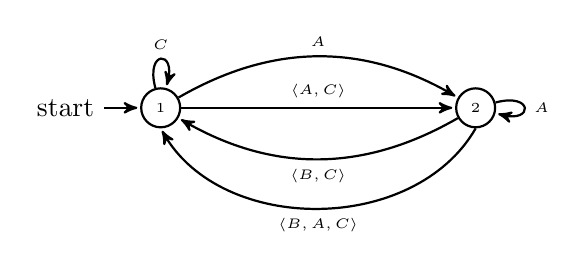
\begin{tikzpicture}[->,>=stealth',shorten >=1pt,auto,node distance=4cm,
  thick,main node/.style={circle,fill=white,draw,font=\sffamily\tiny\bfseries},
  sub node/.style={circle,fill=white,draw,font=\sffamily\tiny\bfseries},
  red node/.style={circle,fill=white,draw,font=\sffamily\tiny\bfseries},
  rec node/.style={rectangle,fill=white,draw,font=\sffamily\tiny\bfseries}]

  \node[initial,main node] (1) [] {$1$};
  \node[main node] (2) [right of=1] {$2$};

 	\path[every node/.style={font=\sffamily\tiny},dashed]
    ;

    \path[every node/.style={font=\sffamily\tiny}]
    (1) edge [bend left] node {$A$} (2)
    (1) edge node {$\langle A,C\rangle$} (2)
    (2) edge [bend left] node {$\langle B, C\rangle$} (1)
    (2.south) edge [bend left=60] node {$\langle B, A, C\rangle$} (1.south)
    (1) edge [loop above] node {$C$} (1)
    %(2) edge [loop above] node {$C$} (2)
    (2) edge [loop right] node {$A$} (2)
    ;

\end{tikzpicture}
\caption{The automata of $c_{B} = c_{A}$ \textbf{delay} $1$ \textbf{on} $c_C$}
\label{delayon}
\end{figure}

$c_B = c_A$ \textbf{DiscretizedBy} $r$ where $r\in \mbb{R}$ creates a discrete-time clock $c_B$. $c_B$ is a subclock of $c_A$.
We define $c_B$ according to a predicate $P \subseteq \mcl{I}_A \times \mcl{I}_B$, which satisfies:

\begin{center}
    $(\forall i\in \mcl{I}_B)(\forall j\in \mcl{I}_A)(\exists d\in \mbb{R}) P(j,i)=true$ iff $\lambda_A(j) = d + (idx_B(i) - 1)\times r$
\end{center}

$c_A$ is an 'ideal clock', denoted as $c_A =$\textbf{IdealClock} iff $\lambda_A: \mcl{I}_A \rightarrow \mbb{R}^+$ is a bijection.

For the detail of binary operations of CCSL, see \cite{andre08}, and for more other information about CCSL, refer to \cite{gascon11}, \cite{mallet13}, \cite{andre09}, \cite{mallet10}, \cite{zaretska} and \cite{UML}.

\subsection{Introduction of Timed Automata~\cite{alur94}}
Properly speaking, well-defined Timed Automata has the same expressive power as deterministic finite automata (DFA), though it gives 'time' as a particular emphasis since it sets real-valued clocks (not to be confused with the CCSL logical clocks) as first-class citizens. A comprehensive study on the expressiveness of various classes of automata can be found in  \cite{diekert08}.

\subsubsection{The Syntax of TA}Let $\mathcal{C}$ be a finite set of non-negative real-valued variables called clocks. The
set of guards $G(\mathcal{C})$ is defined by the grammar $g:=x \bowtie c\ |\ g \wedge g$ where $x \in \mathcal{C}$, $c \in \mathbb{N}$ and $\bowtie \in \{<,\leq,>,\geq,== \}$. A Timed Automata is a tuple $A=(Q,\Sigma,\mathcal{C},q_0,E,I,AP,L,F)$, where:

\begin{itemize}
  \item $Q$ is a finite set of states,
  \item $\Sigma$ is a finite alphabet,
  \item $\mathcal{C}$ is a finite set of clocks,
  \item $q_0 \in Q$ is an initial state,
  \item $E \subseteq Q \times 2^\Sigma \times G(\mathcal{C}) \times 2^{\mathcal{C}} \times Q$ is a finite transition relation,
  \item $I:Q\to G(\mathcal{C})$ is an invariant-assignment function,
  \item $AP$ is a finite set of atomic propositions,
  \item $L:Q \to 2^{AP}$ is a labeling function for the states,
  \item $F \subseteq Q$ is a set of accepting states.
\end{itemize}

\subsubsection{The Operational Semantics of TA} A clock valuation is a function $\nu: \mathcal{C} \to \mathbb{R}$. We define $\nu + r$ as: for
each clock $x \in \mathcal{C}$, $(\nu+r)(x)=\nu(x)+r$, where $r \in \mathbb{R}$. If $Y \subseteq \mathcal{C}$ then a
valuation $\nu[Y := 0]$ is such that for each clock $x \in \mathcal{C} \backslash Y $, $\nu[Y := 0](x) = \nu(x)$ and for each
clock $x \in Y$ , $\nu[Y := 0](x) = 0$. The satisfaction relation $\nu \models g$ for $ g \in G(\mathcal{C})$ is defined in
the natural way.

The operational semantics of a TA $A=(Q,\Sigma,\mathcal{C},q_0,E,I,AP,L,F)$ is a labeled transition system (LTS):
$$
\hookrightarrow_{A}(q,\nu):\ (Q \times \mathbb{T}^{\mathcal{C}})\ \to\ 2^{(Q \times \mathbb{T}^{\mathcal{C}})}
$$

where each mapping determines a transition relation $\langle q,\nu \rangle \to \langle q^\prime,\nu^\prime \rangle$, which is defined as follows:

$$
\hookrightarrow_{A}(q,\nu)=\left\{\begin{array}{ll}
\{\langle q,\nu+\alpha \rangle\} \ \ \  \mbox{if $\exists \alpha \in \mathbb{R}(\nu+\alpha \models I(q)$})\\
\\
\{\langle q^\prime,\nu^\prime \rangle\ |\ q^\prime \in Q^\prime \} \ \ \  \mbox{if $\exists \langle q,A,g,Y,q^\prime \rangle \in E$}\\ \hspace{2.5cm}\mbox{where $\nu \models g$,$\nu^\prime = \nu[Y:=0]$}\\
\\
\{\langle q^\prime,\nu^\prime \rangle\ |\ q^\prime \in Q^\prime \} \cup \{\langle q,\nu+\alpha \rangle\} \ \ \  \mbox{if both}\\

\end{array}\right.
$$

\subsubsection{Transition Relation Function}
The transition relation function $\psi: Q \to 2^{Q}$ is a function over the states
of TA. We declare that for any $q \in Q$, there exists a value of $\psi(q)$ if and only if the set $\{\langle q,A,g,Y,q^\prime\rangle\ |\ \langle q,A,g,Y,q^\prime\rangle \in E\}\neq \emptyset$. For each TA there is a conrrespondent transition relation function.

\section{The Verification Framework of Spatio-Temporal Models }
\ifx
As indicated in the "Introduction" part, a natrual request from the software engineering field is that we wish to use a high-level modeling language to model systems, while applying verification techniques which base on automata theory. So \fi

Classic model checking techniques deals with a formal model $\mathcal{M}$ and specification $\mathcal{\varphi}$ (also called properties). As shown in Fig.~\ref{cvf}, a formal model is usually described with a process algebra like CSP, CCS and Timed CSP, while a formal formula is usually described as a type of modal logic such as LTL, CTL, TCTL, or PSL. Verification by observers (An observer is different from the automata of formal models since it usually contains 'accept states' from which if an error path can be reached,
we say a counter-example that makes our specification failed is found.) consists in building a semantic model for the model, as a transition system, building accepting transition system for the properties and composing both transition systems. The transition system for the property is called an observer since it does not have any side effects. Valid behaviors of the model should always lead to an acceptance state in the observer. Otherwise a counter example can be extracted by exhibiting the 'invalid' path. Different algorithms are applied for different concrete ways of building the observers. For example, the verification of a LTL specification consists in encoding it as a buchi automata, and combining it with the transition system of model by doing cartesian product to be an observer. While the verification of a CTL specification is based on an algorithm that traverses all states of transition system of model based on the syntax structure of CTL.

\begin{figure}[htp]
\centering
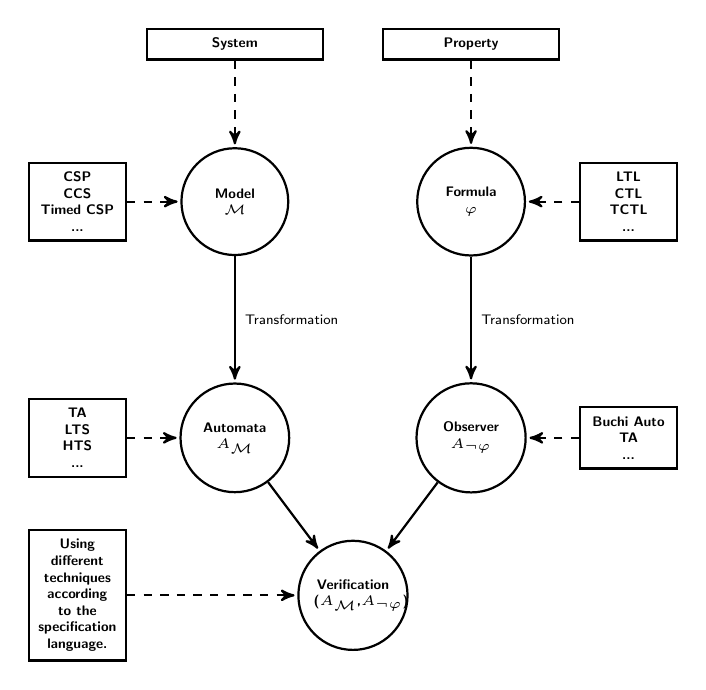
\begin{tikzpicture}[->,>=stealth',shorten >=1pt,auto,node distance=2cm,
  thick,main node/.style={circle,fill=white,draw,font=\sffamily\tiny\bfseries},
  sub node/.style={circle,fill=white,draw,font=\sffamily\tiny\bfseries},
  red node/.style={circle,fill=white,draw,font=\sffamily\tiny\bfseries},
  rec node/.style={rectangle,fill=white,draw,font=\sffamily\tiny\bfseries}]

  \node[rec node] (10) [text width=2cm, align=center] {System};
  \node[rec node] (11) [text width=2cm, align=center,xshift=1cm,right of=10] {Property};
  \node[main node] (1) [text width=1cm, align=center, yshift=0cm,below of=10] {Model\\$\mathcal{M}$};
  \node[main node] (2) [text width=1cm, align=center, yshift=0cm,below of=11] {Formula\\$\mathcal{\varphi}$};
  \node[main node] (3) [text width=1cm, align=center, yshift=-1cm,below of=1]{Automata\\$A_{\mathcal{M}}$};
  \node[main node] (4) [text width=1cm, align=center, yshift=-1cm,below of=2,]{Observer\\$A_{\neg \varphi}$};
  \node[main node] (5) [text width=1cm, align=center, below of=3,xshift=1.5cm] {Verification \\ ($A_\mathcal{M}$,$A_{\neg \varphi}$)};
  \node[rec node] (6) [text width=1cm, align=center, left of=1,xshift=0cm]{CSP \\ CCS \\Timed CSP \\ ...};
  \node[rec node] (7) [text width=1cm, align=center, right of=2,xshift=0cm]{LTL \\ CTL \\ TCTL \\ ...};
  \node[rec node] (8) [text width=1cm, align=center, left of=3,xshift=0cm]{TA \\ LTS \\ HTS \\ ...};
  \node[rec node] (9) [text width=1cm, align=center, right of=4,xshift=0cm]{Buchi Auto \\ TA \\ ...};
  \node[rec node] (12) [text width=1cm,align=center, below of=8]{Using different techniques according to the specification language.};
 	 \path[every node/.style={font=\sffamily\tiny},dashed]
    (10) edge node {} (1)
    (11) edge node {} (2)
    (6) edge node {} (1)
    (7) edge node {} (2)
    (8) edge node {} (3)
    (9) edge node {} (4)
    (12) edge node {} (5);

    \path[every node/.style={font=\sffamily\tiny}]
    (1) edge node {Transformation} (3)
    (2) edge node {Transformation} (4)
    (3) edge node {} (5)
    (4) edge node {} (5);
\end{tikzpicture}
\caption{Classic Verification Framework}
\label{cvf}
\end{figure}

Fig.~\ref{cvf} shows the classic verification framework. Our proposed verification Framework (see Fig.~\ref{nvf}) follows the same scheme but we use STeC for the specification of the model, since it considers both time and locations as first-class citizens, and CCSL as a specification language.
Rather than proposing a direct transformation to transition systems we rather use Timed Automata (TA) as an intermediate formal model. This conveniently allows reusing powerful and widely accepted verification tools like UPPAAL (\cite{alur95} gives basic verification techniques of TA). CCSL has a different expressive power than classical temporal logics (see \cite{gascon11} for a detailed comparison). It offers a set of pre-defined causal and timed patterns that, in our view, helps abstracting fundamental properties on both time and location without having to deal with the full complexity of temporal logics.
 \cite{suryadevara13} describes the family of CCSL specifications that can be encoded as 'pure' Timed Automata. Going through CCSL, compared to describing everything directly as a TA, should alleviate the burden of the design since CCSL provides a library of off-the-shelf often-used property patterns.

\ifx
The classic verification framework shown in Fig.~\ref{cvf} has been developed for many years and is very mature both in theory and application. So we enhance STeC-model to be directly verifiable by transforming it into Timed Automata---a very powerful tool directly support for verification (\cite{alur95} introduces the basic veirification technique of TA).
We introduce a specification language, called CCSL and use it to specify properties of STeC-models.
In CCSL�� the concept of 'clock' of each event was introduced and the complexity logical relations between events are expressed by the composition of such 'clock'. Because of this, some properties are stated in a simpler way using CCSL than using other temporal logic specification languages (such as LTL or CTL). And CCSL in fact is not exactly a subset of PSL \cite{mallet11}. Encoding directly a 'subset' of CCSL into timed automata is not so straightforward, recent work \cite{mallet13} has shown that safe CCSL specifications could be compiled as a timed automaton as a result of the clock calculus process.
\fi
\begin{figure}[htp]
\centering
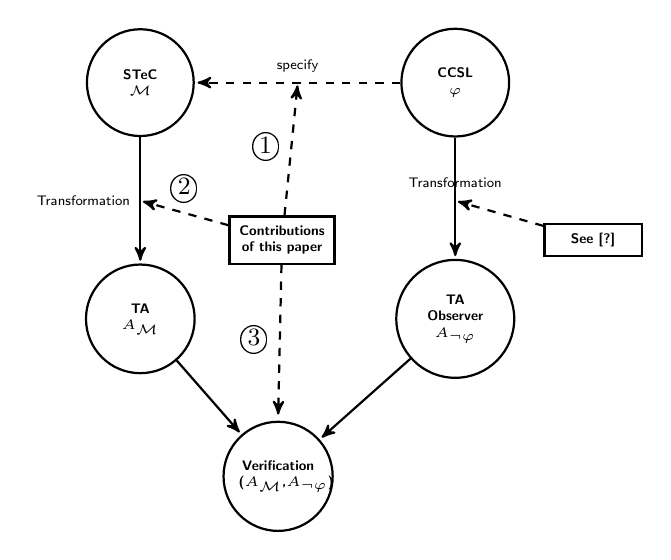
\begin{tikzpicture}[->,>=stealth',shorten >=1pt,auto,node distance=2cm,
  thick,main node/.style={circle,fill=white,draw,font=\sffamily\tiny\bfseries},
  sub node/.style={circle,fill=white,draw,font=\sffamily\tiny\bfseries},
  red node/.style={circle,fill=white,draw,font=\sffamily\tiny\bfseries},
  rec node/.style={rectangle,fill=white,draw,font=\sffamily\tiny\bfseries}]

  %\node[rec node] (10) [text width=2cm, align=center] {System};
  %\node[rec node] (11) [text width=2cm, align=center,xshift=5cm] {Property};
  \node[main node] (1) [text width=1cm, align=center, yshift=0cm] {STeC\\$\mathcal{M}$};
  \node[main node] (2) [text width=1cm, align=center, right of=1,yshift=0cm,xshift=2cm] {CCSL\\$\mathcal{\varphi}$};
  \node[main node] (3) [text width=1cm, align=center, below of=1,yshift=-1cm]{TA\\$A_{\mathcal{M}}$};
  \node[main node] (4) [text width=1cm, align=center, below of=2,yshift=-1cm]{TA Observer\\$A_{\neg \varphi}$};
  \node[main node] (5) [text width=1cm, align=center, below of=3,xshift=1.75cm] {Verification \\ ($A_\mathcal{M}$,$A_{\neg \varphi}$)};
  %\node[rec node] (6) [text width=2cm, align=center, left of=1,xshift=1cm]{CSP \\ CCS \\Timed CSP \\ ...};
  %\node[rec node] (7) [text width=2cm, align=center, right of=2,xshift=-1cm]{LTL \\ CTL \\ TCTL \\ ...};
  %\node[rec node] (8) [text width=2cm, align=center, left of=3,xshift=1cm]{TA \\ LTS \\ HTS \\ ...};
  %\node[rec node] (9) [text width=2cm, align=center, right of=4,xshift=-1cm]{Buchi Auto \\ TA \\ ...};
  %\node[rec node] (12) [text width=3cm,align=center, left of=5]{Using different techniques according to the specification language.};
  \node[rec node] (13) [text width=1.1cm,align=center,below of=1,xshift=1.8cm] {Contributions of this paper};
  \node[rec node] (14) [text width=1cm,align=center,below of=2,xshift=1.75cm] {See \cite{mallet13}};
 	\path[every node/.style={font=\sffamily\tiny},dashed]
    %(10) edge node [dashed] {}(1)
    %(11) edge node {} (2)
    %(6) edge node {} (1)
    %(7) edge node {} (2)
    %(8) edge node {} (3)
    %(9) edge node {} (4)
    %(12) edge node {} (5);
    (2) edge node [above] {specify} (1)
    ;
    \draw [dashed] (13) -- (0cm,-1.5cm) node [midway, above] {\quan{2}};
    \draw [dashed] (14) -- (4cm,-1.5cm);
    \draw [dashed] (13) -- (2cm,0cm) node [midway, left] {\quan{1}};
    \draw [dashed] (13) -- (1.75cm,-4.25cm) node [midway, left] {\quan{3}};
    \path[every node/.style={font=\sffamily\tiny}]
    (1) edge node [left] {Transformation} (3)
    (2) edge node [above] {Transformation} (4)
    (3) edge node {} (5)
    (4) edge node {} (5);
\end{tikzpicture}
\caption{Proposed Verification Framework}
\label{nvf}
\end{figure}


Fig.~\ref{nvf} shows the verification framework we have built in order to verify spatio-temporal specifications of STeC models: i.e., by transforming both STeC and CCSL into Timed Automata(TA). The contributions of this paper are: \quan{1} The definition of CCSL in the domain of STeC. \quan{2} The encoding from STeC into Timed Automata. \quan{3} The implementation of encoding tool from STeC into TA. We will focus on the first two parts. At last we will illustrate the modeling and verification techniques of the proposed verification framework with a simple ITS example.

For the details of the translation from CCSL into TA, see \cite{suryadevara13}.


\ifx
On the other hand, we need to find a specification language for STeC to specify properties in system. Our choice is CCSL(for more details about CCSL, see \cite{mallet11}, \cite{mallet08}, \cite{mallet13}, \cite{mallet1302}, \cite{mallet10}, \cite{galyna} and \cite{andre09}). Because as introduced before, CCSL is easy to express  the logical relationship between two events(in same cases better than LTL).
\fi
\ifx
Another reason of using CCSL as a specification language is that CCSL is a well-defined language and "almost" each formula in CCSL can be mapped to a corresponding TA(see \cite{mallet13}). This result indicates the potential possibility of verifying spatio-temperal specifications of STeC since we can successfully build a "link" between STeC, CCSL and TA. As the Fig.~\ref{GoalOfResearch} shows above, CCSL can be transformed into TA, while $\textcircled{1}$ is what we show later in this paper how to transform STeC into TA. Based on TA, existing verification techniques can be used for the verification of STeC-specifications by combining the transition model--- $\mathcal{M}$ and specification property---$\mathcal{A}_{\varphi}$.

\subsection{CCSL---A specification language}
The Clock Constraint Specification Language is proposed by Frederic Mallet as a
companion language of the UML profile for MARTE \cite{mallet08}.
It is intended to describe the temporal order of events in real-time systems. CCSL is well-defined in its syntax and semantics[11], and it is a specification language which can be transformed into Timed-automata and LTS(\cite{mallet11}, \cite{mallet13}, \cite{mallet1302}). CCSL uses very simple operations to describe profound timed-relationships between two events(such as "precedence", denoted as "$prec$"). Because of these advantages, it is a good choice to use it as a specification language of a formal model of real-time system.
\fi

\ifx
We give a final purpose of our research and list several steps to achieve it:

\paragraph{Our goal} Verifying the STeC-specifications with Timed Automata and using CCSL as a specification language.
\paragraph{Steps}
\begin{enumerate}[i]

\item Build a transformation from STeC to TA.

\item Build a transformation from CCSL to a kind of LTS or TA. This procedure have already been realized. See \cite{mallet13}.%Verifying MARTE/CCSL Mode Behaviors using UPPAAL

\item Define CCSL as a specification language for STeC.

\item Develop a automatic tool for modeling and verification using STeC and CCSL.
\end{enumerate}
\fi

\section{The Definition of CCSL in the Domain of STeC}
From the previous section, we have known that CCSL, as a specification language that offers logic and timed patterns provides a formal semantic support for the verification of UML. Though CCSL is an independent, formal-defined language, but using it as a specification language in the domain of STeC demands some formal definitions. In this section, we import CCSL into the domain of STeC. The definition of CCSL on STeC is quite trivial, so we focus on the explanation of how a STeC formula 'satisfy' a CCSL formula, which builds a connection between CCSL expressions and STeC formulas. For this purpose we firstly give a definition of traces for STeC in a natural way.

\subsection{Traces on STeC}
 As usual done for all process algebra, we define the notion of traces in STeC as a sequence of events (or actions) generated by a STeC model(or say a STeC formula). It can be defined inductively on the structure of STeC expressions.

\begin{mydef}
Denote the set of all processes (formulas) of STeC as:
$$\mathbb{P}_{STeC}=\{\ P\ |\ \mbox{ $P$ is a process in STeC}\}$$

\end{mydef}

\begin{mydef}
The name of an action or an atomic process defined in Section \uppercase\expandafter{\romannumeral2} is called 'alphabet'. For any atomic process of STeC $p$, let $\alpha p$ denote its alphabet. Let $\alpha P$ ($P \in \mathbb{P}_{STeC}$) represent the set of alphabets in process $P$.
\end{mydef}

For example, the alphabet of an atomic process $Send_{(Lapp,t)}(Appr)$ is '$Send$', denoted as $\alpha Send_{(Lapp,t)}(Appr)=Send$.

Another example, let $P = Run(\infty); (Send_{(Lapp,t)}(Appr) \parallel
Approach_{(Lapp,t)}(\Gamma))$. Then $\alpha P = \{Run, Send, Approach\}$ is the set of alphabets of $P$.

\begin{mydef}
An element of trace in STeC, called a STeC word, is a quadruple $e=\langle act,l,t,\delta \rangle$, where $act$ is an atomic process in STeC, $l$ is location, $t$ is time and $\delta$ is the duration time of the action.

$\mathbb{E}_{STeC}$ denotes the set of all elements in STeC.

Define the projection of each item in element $e$ as $\pi_{act}$, $\pi_{l}$, $\pi_{t}$ and $\pi_\delta$ respectively. Generally, let $e=\langle e_1, e_2, ..., e_i, ... \rangle$, we define $\pi_i$ as the projection on the $i$th component of $e$.
\end{mydef}

For example, $\pi_2(\langle e_1, e_2, e_3 \rangle)=e_2$, $\pi_{act}(\langle a_1, l, t, \delta \rangle)=a_1$.

\begin{mydef}
$\mathbf{Words}(P)$ denotes the set of all words of a process $P$.
\end{mydef}

Different from 'actions' in STeC, a 'word' in STeC is a tuple that not only contains the information of the alphabet of an action, but also the location where an action happens, the time at which it occurs and the duration it takes.

For example, let $P = Run(\infty); (\bff{Send}_{(Lapp,t,G)}(Appr) \parallel
Approach_{(Lapp,t)}(\Gamma))$. Then $\mathbf{Words}(P) = \{\langle Run, l_0, t_0, \infty \rangle,\langle \bff{Send}, Lapp, t, 0\rangle,\langle Approach, Lapp, t, \Gamma\rangle \}$.

In this paper, let $f$ is a function, $dom(f)$ denotes the domain of $f$, $im(f)$ denotes the range of $f$, and $graph(f)$ denotes the graph of $f$.

\begin{mydef}
A trace of STeC is a finite or infinite sequence of words which is defined as a partial function $t : \mathbb{N}^{+} \to \mathbb{E}_{STeC}$ ($\mathbb{N}^{+}=\{1,2,3,...\}$ is the set of non-zero natural numbers), where $dom(t) \subseteq \mathbb{N}^{+}$. It is a partial, injective function and satisfies: for any $n \in \mathbb{N}^{+}$, if $n \in dom(t)$, then
$m \in dom(t)$ for all $m < n$.

Let $t_i$ be the $i$th element of trace $t$, we have $t_i=t(i)$. So sometimes we simply write trace $t$ as $t=t_1t_2t_3...$, so for any trace $t$ and $s$, $t=s$ iff $t_i=s_i$ for all $i\in \mbb{N}^+$.


Denote the set of all traces in STeC as $\mathbb{T}_{STeC}$.
\end{mydef}

\begin{mydef}
A binary operator $\frown : \mathbb{T}_{STeC} \times \mathbb{T}_{STeC} \to \mathbb{T}_{STeC}$ concatenates two traces. Let $s$, $t$ be any traces in STeC, $s$ is finite. Set $|dom(s)|=m$, then we have a new trace $r=s \frown t$, which satisfies:
$$for\ all\ x\in \mbb{N}^+,\ \ r(x)=\left\{\begin{array}{ll}
s(x) & \mbox{if $x \le m$}\\
\\
t(x-m) & \mbox{otherwise}\\
\end{array}\right.
$$
\end{mydef}

\begin{mydef}
Let $s,t \in \mathbb{T}_{STeC}$, we denote $s \sqsubseteq t$ when $s$ is a sub trace of t. It satisfies:

\begin{enumerate}[1)]
\item $im(s) \subseteq im(t)$
\item for any $t(i),t(j) \in ran(t)$ and $i \le j$, if there exists $m,n \in \mathbb{N}^+$ such that $s(m)=t(i), s(n)=t(j)$, then $m \le n$ holds.
\end{enumerate}
\end{mydef}

A restriction on trace is a sub trace of it on some specific alphabet set. We have the following definition.

\begin{mydef}
Let $s,t \in \mathbb{T}_{STeC}$, we say $s$ is a restriction of $t$ on an alphabet set $\alpha P$ if and only if $s$ is a sub trace of t where each element belongs to $\alpha P$, denoted as $s=t \upharpoonleft \alpha P$. It satisfies:

\begin{enumerate}[1)]
\item $s \sqsubseteq t$.
\item $im(s)=\{\langle act,l,t,\delta \rangle \ |\ act \in \alpha P\}$.
\end{enumerate}
\end{mydef}

After some preparations, we now give a definition of traces for STeC formulas.

\begin{mydef}
A trace of a STeC formula is a function from the set of STeC formulas to a set of STeC traces, denoted as $\mathbf{Traces}:\mathbb{P}_{STeC} \to \mathbb{T}_{STeC}$. It is defined according to following lows:

\begin{enumerate}[1)]
\itemsep0.05in
\item $\mathbf{Traces}(\mathbf{Stop}^{G}_{(l,t)})=\emptyset$.
\item $\mathbf{Traces}(\bff{Send}^{G \rightharpoonup G^\prime}_{(l,t)}(m))=\{\langle \bff{Send},l,t,0\rangle\}$
\item $\mathbf{Traces}(\bff{Get}^{G \leftharpoonup G^\prime}_{(l,t)}(m))=\{\langle \bff{Get},l,t,0\rangle\}$
\item $\mathbf{Traces}(\bff{\alpha}^{G}_{(l,t)}(l^\prime,\delta))=\{\langle \alpha,l,t,\delta\rangle\}$
\item $\mathbf{Traces}(\bff{\beta}^{G}_{(l,t)}(\delta))=\{\langle \beta,l,t,\delta\rangle\}$
%\item $\mathbf{Traces}(a_{(l,t)} \to P)=\{\langle a,l,t,\delta \rangle \frown t\ |\ t \in Traces(P)\}$.
\item $\mathbf{Traces}(P;Q)=\{s \frown t\ |\ s \in \bff{Traces}(P)\ \wedge\  t \in \bff{Traces}(Q) \}$
\item $\mathbf{Traces}(P\ []\ Q)=\bff{Traces}(P) \cup \bff{Traces}(Q)$
\item $\mathbf{Traces}(P\parallel Q)=\{t\ |\ t \upharpoonleft \alpha P \in \bff{Traces}(P)\ \wedge\ t \upharpoonleft \alpha Q \in \bff{Traces}(Q)\ \wedge\ im(t) \subseteq \alpha P \cup \alpha Q\}$
\item $\mathbf{Traces}(P \unrhd_{\delta} Q)=\{t\ |\ \exists f \exists g \exists k($

    \begin{center}
        $f\in \bff{Traces}(P) $

        $\wedge $

        $g\in \bff{Traces}(Q) $

        $\wedge $

        $\pi_t(t_i)< \delta$ and $\pi_{act}(t_i)=f_i$, for all $i\le k$

        $\wedge$

        $\pi_t(t_i)\ge \delta$ and $\pi_{act}(t_i)=g_{i-k}$, for all $i>k$
    \end{center}

    \ifx
    \begin{center}
    if $\pi_t(t_i)< \delta $, then $\pi_{act}(t_i) \in \alpha P$ and $t_i=f_i$, else $ \pi_{act}(t_i) \in \alpha Q $ and $t_i=g_i $
    \end{center}
    \fi

    $)\}$
\item $\mathbf{Traces}(P \unrhd ([]_{i \in I}A_i \to P_i))=\{t\ |\ \exists f \exists g \exists k \exists i($

    \begin{center}
        $f\in \bff{Traces}(P)$

        $\wedge$

        $g\in \bff{Traces}(P_i)$

        $\wedge$

        $\pi_{act}(t_i)=f_i$, for all $i<k$

        $\wedge$

        $\pi_{act}(t_k)=\alpha A_i$

        $\wedge$

        $\pi_{act}(t_i)=g_{i-k}$, for all $i>k$
    \end{center}

    $)\}$

\item $\mathbf{Traces}(B\to P)=\left\{\begin{array}{ll}
\{t\ |\ \pi_{act}(t_1)=\alpha B \wedge t_2t_3... \in \bff{Traces}(P)\}\ \ \mbox{if $\mathcal{T}(B)=1$}\\
\\
\emptyset \ \ \mbox{otherwise}\\
\end{array}\right.$

\end{enumerate}

See that $[]_{i \in I}B_i \to P_i$ can be easily considered as a special case of $P [] Q$.

\end{mydef}

\subsection{The Definition of CCSL for STeC}
Next let us define the CCSL in the domain of STeC formally according to the definition of STeC traces.

\begin{mydef}
\label{def_clock_stec}
Let $A$ be a set of alphabets in STeC. $c_A=\langle \mathcal{I}, \prec, \lambda, \mathcal{D}\rangle$ is a clock of $A$, which satisfies:
\begin{enumerate}[1)]
\item
    $\mathcal{I}$ is a set of instants, $\prec$ is a quasi-order relation on $\mathcal{I}$ just as defined in the early reference \cite{andre08}

\item
    $\mathcal{D}=A$

\item
    $\lambda : \mathcal{I} \to \mathcal{D}$ is a labelling function. It is a partial, injective function and satisfies that for any $i \in \mathcal{I}$, if $i \in dom(\lambda)$ then for all $j \prec i$, $j \in dom(\lambda)$. This definition is the same as the definition of $\lambda$ in \cite{andre08}.

\ifx
\item
    $\mathcal{F}=\{f_t\ |\ t \in \mathbf{Traces}(P)\}$.
    Set $Idx : \mathbb{N}^+ \to \mathcal{I}$ is a mapping where for each $i \in \mathbb{N}^+$, $Idx(i)$ is the $i$th element of $\mathcal{I}$. For any trace $t \in \mathbf{Traces}(P)$, the function $f_t : \mathcal{I} \to \alpha t$ (where $\alpha t = \{ \pi_{act}(a)\ |\ a \in ran(t)\}$) satisfies that it maps the $i$th instant $Idx(i)$ to the $i$th occurrence of the action, $\lambda(\mathcal{I}(i))$ in trace $t$, that is:
    $$f_t(I) = \pi_{act}(s(Idx^{-1}(I)))$$, where $I \in \mathcal{I}$, $s = t \upharpoonleft A$.
\fi
\end{enumerate}

A clock that satisfies the above rules is said to be in the domain of STeC.

\end{mydef}

In the definition above, the unit of time $\mu$ appearing in the original definition of CCSL in \cite{andre08} is ignored.

\ifx
Since the CCSL in the domain of STeC is just the same as the original one except the unit time $\mu$, so, the definition of binary operators of CCSL are in fact the same as the definition in \cite{mallet08}.
So we have the following declaration.

\begin{mydef}
The definition of the 'Coincidence-based' clock constraint, and the 'Presedence-based' clock constraint which are defined in paper \cite{mallet08} remain the same for the definition of operations of CCSL clock in the domain of STeC.
\end{mydef}
\fi

Next we give the definition of the satisfiability of CCSL formula for a STeC formula.

\begin{mydef}
\label{sat}
$c_A$$=\langle \mathcal{I}, \prec, \lambda, \mathcal{D}\rangle$ is a CCSL clock and $Exp_c$ is an expression obtained by combining clocks using binary operators in CCSL. Then for any traces $t$ (of some process) in STeC,

\begin{enumerate}[1)]
\item $t \models c_A$ iff for any $i\in \mbb{N}^+$, $\pi_{act}((t \upharpoonleft A)(i))=\lambda_i$

\item $t\models c_A\subseteq c_B$ iff $t\upharpoonleft A \models c_A$, $t\upharpoonleft B \models c_B$ and $graph(t\upharpoonleft A)\subseteq graph(t\upharpoonleft B)$

\item $t\models c_A\prec c_B$ iff $t\upharpoonleft A \models c_A$, $t\upharpoonleft B \models c_B$ and $\pi_{t}((t\upharpoonleft A)(i))<\pi_{t}((t\upharpoonleft B)(i))$ for any $i\in \mbb{N}^+$

\end{enumerate}
For any $P\in \mathbb{P}_{STeC}$, $P \models c_A$ (resp. $Exp_c$) iff $t \models c_A$ (resp. $Exp_c$) for all $t\in \mathbf{Traces}(P)$.

\end{mydef}


\section{The Transformation From STeC to TA}
In Section \uppercase\expandafter{\romannumeral3}, we choose TA as an intermediate model for the model checking of STeC model because in this way, we can make full use of developed verification tools like UPPAAL. In this section, we mainly focus on the transformation from STeC to TA. We want to build a deductive mapping on the structure of STeC expressions. But firstly, we have to introduce three binary operations
over TAs to ease the building of complex TAs by composing simpler ones.

%In this section, we do NOT consider the binary operation
\subsection{New Binary Operators for Timed Automata}

Firstly, we introduce some binary operations on TAs, which are essential for the transformation from STeC to TA.

\subsubsection{STeC-Sequence} We introduce a binary operator over TAs, denoted as $\diamond_{STeC}$. Informally, it 'concatenates' two TAs by adding transitions from one's each final states to the other's initial state. This operator is essential for the sequential composition in STeC (P;Q), see Def.~\ref{def_stec_to_ta}.
\begin{mydef}
Let $A=(Q,\Sigma,\mathcal{C},q_0,E,I,AP,L,F)$ and  $A^\prime=(Q^\prime,\Sigma^\prime,\mathcal{C}^\prime,q_0^\prime,E^\prime,I^\prime,AP^\prime,L^\prime,F^\prime)$ be two TAs.
We introduce a binary operator over TAs called "STeC-Sequence" and defined as follows:

$$\diamond_{STeC}:\ \mathbf{TA} \times \mathbf{TA} \ \to \ \mathbf{TA}$$ where $\mathbf{TA}$ represents the set of all TAs.
Let $A^{\prime\prime}=(Q^{\prime\prime},\Sigma^{\prime\prime},\mathcal{C}^{\prime\prime},q_0^{\prime\prime},E^{\prime\prime},I^{\prime\prime},AP^{\prime\prime},
L^{\prime\prime},F^{\prime\prime})$ such that $A^{\prime\prime}=A \diamond_{STeC} A^\prime$ and it satisfies:

\begin{itemize}
\item $A^{\prime\prime}=(Q \cup Q^{\prime},\Sigma \cup \Sigma^{\prime},\mcl{C}\cup \mcl{C^\prime}\cup \{y\},q_0,E^{\prime\prime},I^{\prime\prime},AP \cup AP^{\prime},
L\cup L^\prime,F^{\prime})$, where $y$ is a new clock.

\item $E^{\prime\prime}=$ $E \cup E^\prime \cup $ $\{$ $\langle f, \emptyset, y==0, \{y\}, i\rangle\ |\ $
    $f\in F$ $\wedge$ $i=q^\prime_0$ $\}$

\item $I^{\prime\prime}$ is defined as follows:

$$I^{\prime\prime}(q)=\left\{\begin{array}{ll}
I(q)\wedge y\le 0 \ \ \  \mbox{if $q \in F$}\\
\\
I(q) \ \ \  \mbox{if $q \in Q \wedge \{q\} \cap F = \emptyset$}\\
\\
I^\prime(q) \ \ \  \mbox{otherwise}\\
\end{array}\right.
$$


\ifx
\item The transition relation function
$\psi^{\prime\prime}(q)$ is defined as:

$$\psi^{\prime\prime}(q)=\left\{\begin{array}{ll}
\psi(q) \ \ \  \mbox{if $q \in Q \wedge \{q\} \cap F = \emptyset$}\\
\\
\psi(q) \cup \psi^\prime(q_0^\prime) \ \ \  \mbox{if $q \in Q \wedge \{q\} \cap F \neq \emptyset$}\\
\hspace{2.5cm}                           \mbox{OR $q \in Q^\prime \wedge q=q_0^\prime$}\\
\\
\psi^\prime(q) \ \ \  \mbox{if $q \in Q^\prime \cap q \neq q_0^\prime$}\\
\end{array}\right.
$$

\item The labelling function $L^{\prime\prime}$ is defined as:

$$
L^{\prime\prime}(q)=\left\{\begin{array}{ll}
L(q) \ \ \  \mbox{if $q \in Q \wedge q \notin F$}\\
\\
L(q) \cup L^\prime(q_0^\prime) \ \ \  \mbox{if $q \in F$}\\
\hspace{2.5cm} \mbox{OR $q \in Q^\prime \wedge q = q_0^\prime$}\\
\\
L^\prime(q) \ \ \  \mbox{if $q \in Q^{\prime} \wedge q \neq q_0^\prime$}\\
\end{array}\right.
$$
\fi
\end{itemize}
\label{TAseq}
\end{mydef}

\subsubsection{STeC-Choice}The second introduced binary operator over TAs serves to build the choice operation in STeC. Informally, it combines two TAs by adding a new state, and two transitions from it to the initial states of each TA. It is called 'STeC-Choice' and denoted as $\oplus_{STeC}$.

\begin{mydef}
Let $A=(Q,\Sigma,\mathcal{C},q_0,E,I,AP,L,F)$, $A^\prime=(Q^\prime,\Sigma^\prime,\mathcal{C}^\prime,q_0^\prime,E^\prime,I^\prime,AP^\prime,L^\prime,F^\prime)$ be two TAs. Define
$$\oplus_{STeC}:\ \mathbf{TA} \times \mathbf{TA} \to \mathbf{TA}$$
as the "STeC-Choice" where:

\begin{itemize}
\item
Let $A^{\prime\prime}=A \oplus_{STeC} A^{\prime}$, then $A^{\prime\prime}=(Q \cup Q^{\prime} \cup \{q_0^{\prime\prime}\},\Sigma \cup \Sigma^{\prime}, \mcl{C}\cup \mcl{C^\prime}\cup \{y\},q_0^{\prime\prime},E^{\prime\prime}, I^{\prime\prime}, AP \cup AP^{\prime},
L\cup L^\prime,F \cup F^{\prime})$, where $y$ is a new clock.

\item $E^{\prime\prime}=$ $E\cup E^\prime \cup$ $\{$
        $\langle q^{\prime\prime}_0, \emptyset, y=0, \{y\}, q_0\rangle$ $, $
        $\langle q^{\prime\prime}_0, \emptyset, y=0, \{y\}, q^\prime_0\rangle\}$

\item $I^{\prime\prime}=I\cup I^\prime \cup \{\langle q^{\prime\prime}_0, y\le0\rangle\}$

\ifx
\item We define the transition relation function $\psi^{\prime\prime}$.
$\psi^{\prime\prime}(q)$ is defined as:

$$\psi^{\prime\prime}(q)=\left\{\begin{array}{ll}
\psi(q) & \mbox{if $q \in Q $}\\
\\
\psi^\prime(q) & \mbox{if $q \in Q^\prime$}\\
\\
\{q_0,q_0^\prime\} & \mbox{if $q = q_0^{\prime\prime}$}\\
\end{array}\right.
$$

\item The labelling function $L^{\prime\prime}$ is defined as:

$$
L^{\prime\prime}(q)=\left\{\begin{array}{ll}
L(q) & \mbox{if $q \in Q $}\\
\\
L^\prime(q) & \mbox{if $q \in Q^{\prime}$}\\
\\
\emptyset & \mbox{if $q = q_0^{\prime\prime}$}\\
\end{array}\right.
$$

\item The invariant-assignment function $I^{\prime\prime}$ is defined as:

$$
I^{\prime\prime}(q)=\left\{\begin{array}{ll}
I(q) & \mbox{if $q \in Q $}\\
\\
I^\prime(q) & \mbox{if $q \in Q^{\prime}$}\\
\\
\{y \leq 0\} & \mbox{if $q = q_0^{\prime\prime}$}\\
\end{array}\right.
$$
\fi

\end{itemize}
\label{TAcho}
\end{mydef}
\subsubsection{STeC-Parallel}The third operation is called "STeC Parallel" which serves to build the parallel operation in STeC. Informally, it is like the 'Hand Shaking' operator defined over transition systems, combing two TAs by doing cartesian product. It is denoted as $\otimes_{STeC}$.

\begin{mydef}
Knowing $A=(Q,\Sigma,\mathcal{C},q_0,E,I,AP,L,F)$, $A^\prime=(Q^\prime,\Sigma^\prime,\mathcal{C}^\prime,q_0^\prime,E^\prime,I^\prime,AP^\prime,L^\prime,F^\prime)$ are two TAs. The definition of
"STeC-Parallel" is given as follows:
$$\otimes_{STeC}:\ \mathbf{TA} \times \mathbf{TA} \to \mathbf{TA}$$
let $A^{\prime\prime}=A \otimes_{STeC} A^{\prime}$, $A^{\prime\prime}$ is defined as follows:

\begin{itemize}
\item
$A^{\prime\prime}=(Q \times Q^{\prime},\Sigma \cup \Sigma^{\prime},\{x,y\},\langle q_0, q_0^{\prime} \rangle,E^{\prime\prime}, I^{\prime\prime},AP \cup AP^{\prime},
L^{\prime\prime},F \times F^{\prime})$

\item $E^{\prime\prime}=E_1 \cup E_2 \cup E_3 \cup E_4$, where:
\begin{enumerate}[1)]
    \item $E_1=$ $\{$ $\langle \langle q_1,q_2\rangle, \{m\}, g_1\wedge g_2, Y_1\cup Y_2, \langle q^\prime_1, q^\prime_2\rangle \rangle\ |$

    \begin{center}
    ($\langle q_1,\{m!\},g_1,Y_1,q^\prime_1\rangle \in E$ $\wedge$

    $\langle q_2,\{m?\},g_2,Y_2,q^\prime_2\rangle \in E^\prime$)

    $\vee$

    ($\langle q_1,\{m?\},g_1,Y_1,q^\prime_1\rangle \in E$ $\wedge$

    $\langle q_2,\{m!\},g_2,Y_2,q^\prime_2\rangle \in E^\prime$)

    \end{center}

    $\}$

    \item $E_2=$ $\{$ $\langle \langle q_1,q_2\rangle, A_1\cup A_2, g_1\wedge g_2, Y_1\cup Y_2, \langle q^\prime_1, q^\prime_2\rangle \rangle\ |$

    \begin{center}
    $\langle q_1,A_1,g_1,Y_1,q^\prime_1\rangle \in E$

    $\wedge$

    $\langle q_2,A_2,g_2,Y_2,q^\prime_2\rangle \in E^\prime$

    \end{center}

    $\}$

    \item $E_3=$ $\{$ $\langle \langle q_1,q_2\rangle, A_1, g_1, Y_1, \langle q^\prime_1, q_2\rangle \rangle\ |$

    \begin{center}
    $\langle q_1,A_1,g_1,Y_1,q^\prime_1\rangle \in E$

    \end{center}

    $\}$

    \item $E_4=$ $\{$ $\langle \langle q_1,q_2\rangle, A_2, g_2, Y_2, \langle q_1, q_2^\prime\rangle \rangle\ |$

    \begin{center}
    $\langle q_2,A_2,g_2,Y_2,q^\prime_2\rangle \in E^\prime$

    \end{center}

    $\}$
\end{enumerate}

'$m!$' and '$m?$' are two special alphabets that will be defined in Def.~\ref{def_stec_to_ta}, here we can simply take them as normal alphabet names in TA.

\ifx
\item Define the transition relation function $\psi^{\prime\prime}$.
$\psi^{\prime\prime}(\langle q_1,q_2 \rangle)$ is defined as:
$$\psi^{\prime\prime}(\langle q_1,q_2\rangle)=$$
$$\left\{\begin{array}{ll}
\langle \psi(q_1),\psi^\prime(q_2) \rangle \ \ \  \mbox{if $\langle q_1,q_2\rangle \in Q \times Q^\prime\ \wedge\ $}\\
\hspace{2.5cm}\mbox{$\exists \langle q_1,m!,g,Y,Q \rangle \in E$ and }\\
\hspace{2.5cm}\mbox{$\exists \langle q_2,m?,g^\prime,Y^\prime,Q^\prime \rangle \in E^\prime$}\\
\hspace{2.5cm}\mbox{OR}\\
\hspace{2.5cm} \mbox{$\exists \langle q_1,m?,g,Y,Q \rangle \in E$ and}\\
\hspace{2.5cm}\mbox{$\exists \langle q_2,m!,g^\prime,Y^\prime,Q^\prime \rangle \in E^\prime$ }\\
\\
\{\ \langle \psi(q_1),\psi^\prime(q_2) \rangle, \langle \psi(q_1),q_2\rangle, \langle q_1, \psi(q_2)\rangle\ \}\\
\hspace{2.5cm}\mbox{if $\langle q_1,q_2\rangle \in Q \times Q^\prime\ \wedge\ $}\\
\hspace{2.5cm}\mbox{$\exists \langle q_1,a,g,Y,Q \rangle \in E$ and }\\
\hspace{2.5cm}\mbox{$\exists \langle q_2,a^\prime,g^\prime,Y^\prime,Q^\prime \rangle \in E^\prime$}\\
\\
\langle \psi(q_1),q_2 \rangle \ \ \ \mbox{if $\langle q_1,q_2\rangle \in Q \times Q^\prime\ \wedge\ $}\\
\hspace{2.5cm} \mbox{$\exists \langle q_1,a,g,Y,Q \rangle \in E$}\\
\\
\langle q_1,\psi(q_2) \rangle \ \ \  \mbox{if $\langle q_1,q_2\rangle \in Q \times Q^\prime\ \wedge\ $}\\
\hspace{2cm} \mbox{$\exists \langle q_2,a^\prime,g^\prime,Y^\prime,Q^\prime \rangle \in E^\prime$}\\
\end{array}\right.
$$

where $m$ is any message in STeC.
\fi

\item $L^{\prime\prime}$ is defined as:
$$
L^{\prime\prime}(\langle q_1,q_2 \rangle)=
L(q_1)\ \cup\ L^\prime(q_2)\ \ \mbox{for all $\langle q_1,q_2\rangle \in Q \times Q^\prime$}
$$

\item $I^{\prime\prime}$ is defined as:
$$
I^{\prime\prime}(\langle q_1,q_2 \rangle)=I(q_1)\ \cup\ I^\prime(q_2)\ \ \mbox{for all $\langle q_1,q_2\rangle \in Q \times Q^\prime$}
$$

\end{itemize}
\label{TApar}
\end{mydef}


\subsection{From SteC to TA: Induction on the Structure of STeC Specification}
After the essential operators have been defined, we can now define a mapping from STeC to TA. We need to define a homomorphism from the set of language STeC to the set of TA inductively.

\begin{mydef}
Denote the set of all TAs as:
$$
\mathbb{M}_{TA}=\{\ A\ |\ \mbox{$A$ is a Timed Automata}\}
$$

\end{mydef}

\begin{mydef}
Knowing that $\mathbb{P}_{STeC}$ and $\mathbb{M}_{TA}$ are the sets of formulas of STeC and TA respectively. We define a homomorphism $\mathcal{F}:\mathbb{P}_{STeC} \rightarrow \mathbb{M}_{TA}$ which can be inductively built according to the following rules:

%\renewcommand{\labelenumii}{\labelenumi\alph{enumii}) }
%\renewcommand{\theenumi}{\roman{enumi}}
%\renewcommand{\labelenumi}{\alph{enumi})}
\begin{enumerate}[i)]
\itemsep0.05in
\item
$\mathcal{F}(\mathbf{Send}^{G \rightharpoonup G^\prime}_{(l,t)}(m))=$

\begin{center}
$
(\{q_0,q_1\},\{m!\},\{x,y\},q_0,E,I,AP,L,\{q_1\})
$.

\end{center}

$E=\{\langle q_0,\{m!\},\{x==t\},\{y\},q_1 \rangle\}$. $x==t$ is a guard, meaning that only when the global clock $x$ equals $t$, transition is fired.

$I=\emptyset$.

$AP=\{l\}$.

$L = \{\langle q_0, l\rangle, \langle q_1, l\rangle\}$.

Fig.~\ref{TAOfSend} shows the graph of the TA.

\ifx
\begin{figure}[htp]
\centering
\includegraphics[scale=0.5]{graph/SEND.png}
\caption{the TA of $\mathbf{Send}^G_{(l,t,G^\prime)}(m)$}
\end{figure}
\fi

\begin{figure}[htp]
\centering
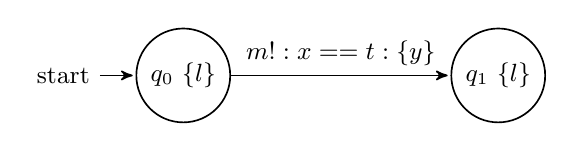
\begin{tikzpicture}[->,>=stealth',shorten >=1pt,auto,node distance=4cm,
                    semithick]
  \tikzstyle{every state}=[text=black,minimum size=0pt]
  	\tikzstyle{every node}=[font=\small,minimum size=0pt]
\node [initial,state] (0) {$q_0$ $\{l\}$};
\node [state] [right of=0] (1) {$q_1$ $\{l\}$};

\path (0) edge node {$m!:x==t:\{y\}$} (1);

	\end{tikzpicture}
\caption{The TA of $\mathbf{Send}^{G \rightharpoonup G^\prime}_{(l,t)}(m)$}
\label{TAOfSend}
\end{figure}

\item
$\mathcal{F}(\mathbf{Get}^{G \leftharpoonup G^\prime}_{(l,t)}(m))=$

\begin{center}
$(\{q_0,q_1\},\{m?\},\{x,y\},q_0,E,I,AP,L,\{q_1\})
$.
\end{center}

$E=\{\langle q_0,\{m?\},\{x==t\},\{y\},q_1 \rangle\}$.

$I=\emptyset$.

$AP=\{l\}$.

$L = \{\langle q_0, l\rangle, \langle q_1, l\rangle\}$.


Fig.~\ref{TAOfGet} shows the TA of $\mathbf{Get}^{G \leftharpoonup G^\prime}_{(l,t)}(m)$.

\ifx
\begin{figure}[htp]
\centering
\includegraphics[scale=0.5]{graph/GET.png}
\caption{the TA of $\mathbf{Get}^{G \leftharpoonup G^\prime}_{(l,t)}(m)$}
\end{figure}
\fi

\begin{figure}[htp]
\centering
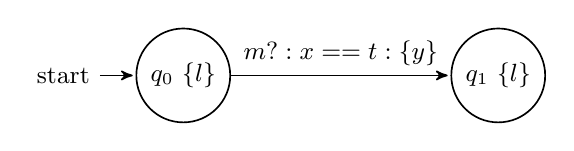
\begin{tikzpicture}[->,>=stealth',shorten >=1pt,auto,node distance=4cm,
                    semithick]
  \tikzstyle{every state}=[text=black,minimum size=0pt]
  	\tikzstyle{every node}=[font=\small,minimum size=0pt]
\node [initial,state] (0) {$q_0$ $\{l\}$};
\node [state] [right of=0] (1) {$q_1$ $\{l\}$};

\path (0) edge node {$m?:x==t:\{y\}$} (1);

	\end{tikzpicture}
\caption{The TA of $\mathbf{Get}^{G \leftharpoonup G^\prime}_{(l,t)}(m)$}
\label{TAOfGet}
\end{figure}

\item
$
\mathcal{F}(\alpha^{G}_{(l,t)}(l^{\prime},\delta))=$

\begin{center}
$(\{q_0,q_1\},\{\alpha\},\{x,y\},q_0,E,I,AP,L,\{q_1\})
$.
\end{center}

$E=\{\langle q_0,\{\alpha\},x==t+\delta \wedge y== \delta,\{y\},q_1 \rangle\}$.

$I=\{\langle q_0, y\leq \delta\rangle\}$.

$AP=\{l,l^\prime\}$.

$L=\{\langle l, q_0\rangle, \langle l^\prime, q_1\rangle\}$.

Fig.~\ref{TAOfAlpha} shows the TA of $\alpha^{G}_{(l,t)}(l^{\prime},\delta)$.

\ifx
\begin{figure}[htp]
\centering
\includegraphics[scale=0.5]{graph/ALPHA.png}
\caption{the TA of $\alpha^{G}_{(l,t)}(l^{\prime},\delta)$}
\end{figure}
\fi

\begin{figure}[htp]
\centering
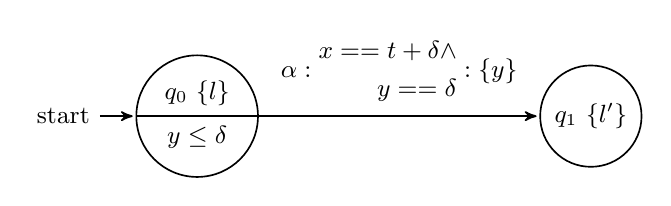
\begin{tikzpicture}[->,>=stealth',shorten >=1pt,auto,node distance=5cm,
                    semithick]
\tikzstyle{every state}=[text=black,minimum size=0pt]
  	\tikzstyle{every node}=[font=\small,minimum size=0pt]
\node [initial,state with output] (0) {$q_0$ $\{l\}$ \nodepart{lower} $y \le \delta$};
\node [state] [right of=0] (1) {$q_1$ $\{l^\prime\}$};

\path (0) edge node {$\alpha:\begin{aligned}x==t+\delta \wedge \\ y== \delta\end{aligned}:\{y\}$} (1);

	\end{tikzpicture}
\caption{The TA of $\alpha^{G}_{(l,t)}(l^{\prime},\delta)$}
\label{TAOfAlpha}
\end{figure}

\item
$
\mathcal{F}(\beta^{G}_{(l,t)}(\delta))=
$

\begin{center}
$
    (\{q_0\},x==t+\delta,\{x,y\},q_0,E,I,AP,L,\{q_0\})
$.
\end{center}

$E=\langle q_0,\{\alpha\},x==t+\delta \wedge y==\delta,\{y\},q_0 \rangle$.

$I=\{\langle q_0, y\leq \delta\rangle\}$.

$AP=\{l\}$.

$L=\{\langle q_0, l\rangle\}$.

Fig.~\ref{TAOfBeta} shows the corresponding TA.

\ifx
 \begin{figure}[htp]
\centering
\includegraphics[scale=0.5]{graph/BETA.png}
\caption{the TA of $\beta^{G}_{(l,t)}(\delta)$}
\end{figure}
\fi

\begin{figure}[htp]
\centering
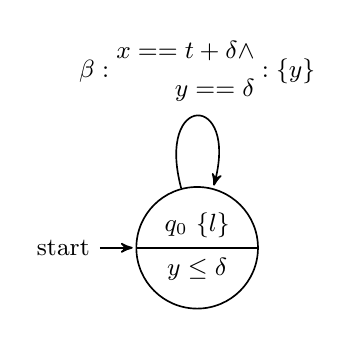
\begin{tikzpicture}[->,>=stealth',shorten >=1pt,auto,node distance=5cm,
                    semithick]
\tikzstyle{every state}=[text=black,minimum size=0pt]
  	\tikzstyle{every node}=[font=\small,minimum size=0pt]
\node [initial,state with output] (0) {$q_0$ $\{l\}$ \nodepart{lower} $y \le \delta$};

\path (0) edge [loop above] node {$\beta:\begin{aligned}x==t+\delta \wedge \\ y==\delta\end{aligned}:\{y\}$} (0);

	\end{tikzpicture}

\caption{The TA of $\beta^{G}_{(l,t)}(\delta)$}

\label{TAOfBeta}
\end{figure}

\ifx
\item
Let $a$ is an atomic process $A$ or $B$. Then:
$$\mathcal{F}(a \to P)=\mathcal{F}(a) \diamond_{STeC} \mathcal{F}(P)$$
\fi

\item
For all $R \in \mathbb{P}_{STeC}$, if $R = P\ ;\ Q$, then

$$\mathcal{F}(R)=\mathcal{F}(P;Q)=\mathcal{F}(P) \diamond_{STeC} \mathcal{F}(Q)$$

where $\diamond_{STeC}$ is the 'STeC-Sequence' operator over TAs defined in Def.~\ref{TAseq}.

Fig.~\ref{PAndQ} shows the TA of $P$ and $Q$ respectively. Fig.~\ref{pseqq} shows the TA of $P;Q$, where $i_P$, $i_Q$ are the initial state of $\mcl{F}(P)$ and $\mcl{F}(Q)$ respectively. $f_P$, $f_Q$ are the final state of $\mcl{F}(P)$ and $\mcl{F}(Q)$ respectively. More than one final state is allowed.

\ifx
 \begin{figure}[htp]
\centering
\includegraphics[scale=0.5]{graph/P_Q.png}
\caption{the TA of $P$ and $Q$}
\end{figure}
\fi

\begin{figure}[htp]
\centering
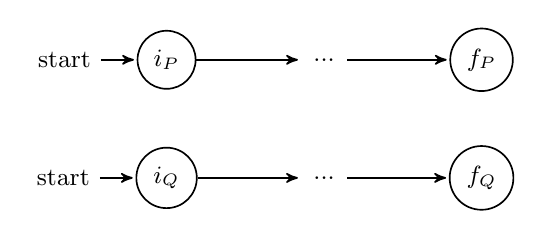
\begin{tikzpicture}[->,>=stealth',shorten >=1pt,auto,node distance=2cm,
                    semithick]
\tikzstyle{every state}=[text=black,minimum size=0pt]
  	\tikzstyle{every node}=[font=\small,minimum size=0pt]
\node [initial,state] (0) {$i_P$};
\node [state] [right of=0,draw=none] (1) {$...$};
\node [state] [right of=1] (2) {$f_P$};

\node [initial,state] [below of=0,yshift=0.5cm] (3) {$i_Q$};
\node [state] [right of=3,draw=none] (4) {$...$};
\node [state] [right of=4] (5) {$f_Q$};

\path (0) edge node {} (1)
	   (1) edge node {} (2)
	
	   (3) edge node {} (4)
	   (4) edge node {} (5);

	\end{tikzpicture}
	
	\ifx
	\includegraphics[width=2.5in]{graph/PAndQ.png}
	\fi
\caption{The TA of $P$ and $Q$}
\label{PAndQ}
\end{figure}

\ifx
 \begin{figure*}[!t]
\centering
\includegraphics[width=2.5in]{graph/SEQ.png}
\caption{the TA of $P;Q$}
\label{PSeqQ}
\end{figure}
\fi

\begin{figure}[htp]
\centering
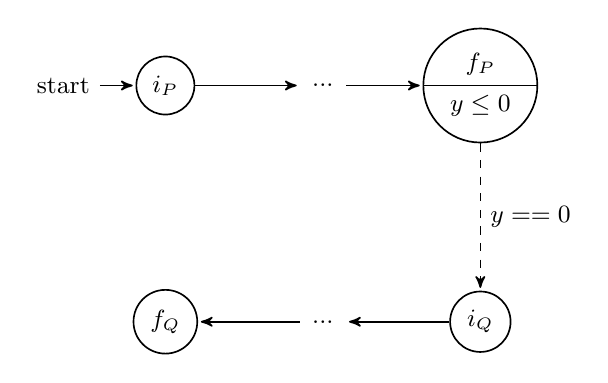
\begin{tikzpicture}[->,>=stealth',shorten >=1pt,auto,node distance=2cm,
                    semithick]
\tikzstyle{every state}=[text=black,minimum size=0pt]
  	\tikzstyle{every node}=[font=\small,minimum size=0pt]
\node [initial,state] (0) {$i_P$};
\node [state] [right of=0,draw=none] (1) {$...$};
\node [state] [right of=1,state with output] (2) {$f_P$ \nodepart{lower} $y\le0$};
\node [state] [below of=2,yshift=-1cm] (5) {$i_Q$};
\node [state] [left of=5,draw=none] (3) {$...$};
\node [state] [left of=3] (4) {$f_Q$};

\path (0) edge node {} (1)
	   (1) edge node {} (2)
	   (5) edge node {} (3)
	   (3) edge node {} (4);
\path[every node/.style={font=\sffamily\small},dashed]
    (2) edge node {$y==0$} (5);

	\end{tikzpicture}
	
	\ifx
	\includegraphics[width=2.5in]{graph/PseqQ.png}
	\fi
\caption{The TA of $P;Q$}
\label{pseqq}
\end{figure}

\item
$$\mathcal{F}(B \to P)=\left\{\begin{array}{ll}
\mathcal{F}(B)\diamond_{STeC} \mathcal{F}(P) & \mbox{if $\mathcal{T}(B)=1$}\\
\\
\emptyset & \mbox{otherwise}\\
\end{array}\right.
$$

\item
For all $R \in \mathbb{P}_{STeC}$, if $R = P\ []\ Q$, then
$$\mathcal{F}(R)=\mathcal{F}(P\ []\ Q)=\mathcal{F}(Q) \oplus_{STeC} \mathcal{F}(P)$$
%$$=A_Q \oplus_{STeC} A_P$$

where $\oplus_{STeC}$ is the 'STeC-Choice' operator over TAs defined in Def.~\ref{TAcho}.

Fig.~\ref{PChiQ} shows the TA of $P[]Q$, of which the initial state is the 'new' state.

\ifx
 \begin{figure}[htp]	
\centering
\includegraphics[scale=0.5]{graph/CHO.png}
\caption{the TA of $P[]Q$}
\end{figure}
\fi

\begin{figure}[htp]
\centering

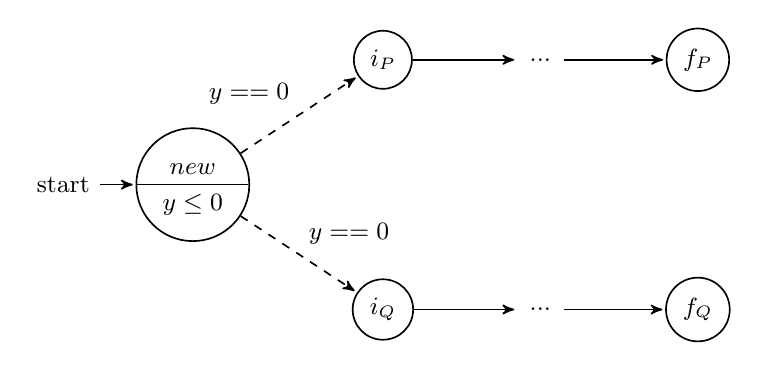
\begin{tikzpicture}[->,>=stealth',shorten >=1pt,auto,node distance=2.0cm,
                    semithick]
\tikzstyle{every state}=[text=black,minimum size=0pt]
  	\tikzstyle{every node}=[font=\small,minimum size=0pt]
\node [initial,state with output] (0) {$new$ \nodepart{lower} $y\le0$};
\node [state] [above right of=0, yshift=-3cm,xshift=1cm] (1) {$i_Q$};
\node [state] [right of=1,draw=none] (2) {$...$};
\node [state] [right of=2] (3) {$f_Q$};
\node [state] [below right of=0, yshift=3cm,xshift=1cm] (4) {$i_P$};
\node [state] [right of=4,draw=none] (5) {$...$};
\node [state] [right of=5] (6) {$f_P$};

\path
	   (1) edge node {} (2)
	   (2) edge node {} (3)
	   (4) edge node {} (5)
      (5) edge node {} (6);

\path[every node/.style={font=\sffamily\small},dashed]
        (0) edge node {$y==0$} (1)
	    (0) edge node {$y==0$} (4)
    ;

	\end{tikzpicture}
	
	
	%\includegraphics[width=2.5in]{graph/PparQ.png}
\caption{The TA of $P[]Q$}
\label{PChiQ}
\end{figure}

\item
For all $R \in \mathbb{P}_{STeC}$, if $R = P\ \parallel \ Q$, then
$$\mathcal{F}(R)=\mathcal{F}(P\ \parallel \ Q)=\mathcal{F}(Q) \otimes_{STeC} \mathcal{F}(P)$$
%$$=A_Q \otimes_{STeC} A_P$$

where $\otimes_{STeC}$ is the 'STeC-Parallel' operator over TAs defined in Def.~\ref{TApar}. And Fig.~\ref{PParQ} shows the corresponding TA.


\ifx
 \begin{figure}[htp]
\centering
\includegraphics[scale=0.5]{graph/PAR.png}
\caption{the TA of $P \parallel Q$}
\end{figure}
\fi

\begin{figure}[htp]
\centering
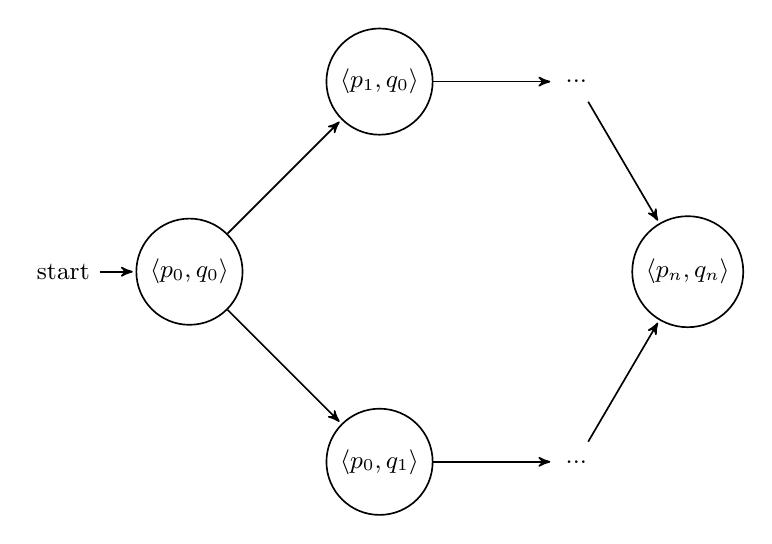
\begin{tikzpicture}[->,>=stealth',shorten >=1pt,auto,node distance=2cm,
                    semithick]
\tikzstyle{every state}=[text=black,minimum size=0pt]
  	\tikzstyle{every node}=[font=\small,minimum size=0pt]
\node [initial,state] (0) {$\langle p_0,q_0\rangle$};
\node [state] [above right of=0, yshift=1cm,xshift=1cm] (1) {$\langle p_1,q_0\rangle$};
\node [state] [right of=1,xshift=0.5cm,draw=none] (2) {$...$};
\node [state] [below right of=0, yshift=-1cm,xshift=1cm] (3) {$\langle p_0,q_1\rangle$};
\node [state] [right of =3,xshift=0.5cm,draw=none] (4) {$...$};
\node [state] [above right of=4,yshift=1cm] (5) {$\langle p_n,q_n \rangle$};

\path (0) edge node {} (1)
	  (0) edge node {} (3)
	   (1) edge node {} (2)
	   (2) edge node {} (5)
		(3) edge node {} (4)
	   (4) edge node {} (5);
	\end{tikzpicture}
\caption{The TA of $P \parallel Q$}
\label{PParQ}
\end{figure}

\ifx
\item
For any process $R\ =\ P \unrhd_{\delta} Q$, we consider to convert it into a form which contains only the operator "$[]$" and "$\to$".

If $P=\mathbf{Stop}$, it is easy to see that $P \unrhd_{\delta} Q = Q$. So set $P=a\to P^\prime$, $a$ can be any atomic process type $A$ or $B$. We decompose $P \unrhd_{\delta} Q$ in the following way:
$$
P \unrhd_{\delta} Q=\left\{\begin{array}{ll}
a \to (P^\prime \unrhd_{\delta - \tau(a)} Q) & \mbox{if $\delta-\tau(a)>0$}\\
\\
(a \to (P^\prime \unrhd Q))[]Q & \mbox{otherwise}\\
\end{array}\right.
$$

So in fact, $P \unrhd_{\delta} Q$ can be replaced by a formula in which only operator '$\to$' and '$[]$' are used.
\fi

\item Let $\mathcal{F}(P \unrhd_{\delta} Q)=(Q,\Sigma,\mathcal{C},q_0,E,I,AP,L,F)=\mathcal{F}(P) \curvearrowright_\delta \mathcal{F}(Q)$, $\curvearrowright_\delta$ is a binary operator over TAs. Let $\mathcal{F}(P)=(Q_P,\Sigma_P,\mathcal{C}_P,s_P,E_P,I_P,AP_P,L_P,F_P)$ and
    $\mathcal{F}(Q)=(Q_Q,\Sigma_Q,\mathcal{C}_Q,s_Q,E_Q,I_Q,AP_Q,L_Q,F_Q)$. We define $\curvearrowright_\delta$ as follows:
    \begin{itemize}
        \item $Q=Q_P \cup Q_Q$
        \item $\Sigma=\Sigma_P \cup \Sigma_Q$
        \item $\mathcal{C}=\mcl{C}_P \cup \mcl{C}_Q \cup \{x\}$. $x$ is a new clock
        \item $q_0=i_P$ where $i_P$ is the initial state of $\mathcal{F}(P)$
        \item $AP=AP_P \cup AP_Q$
        \item $L=L_P \cup L_Q$
        \item $F=F_Q$
        \item $I=I_P \cup I_Q \cup$$\{\langle q,x\le \delta\rangle\ |\ $ $q\in Q_P\}$
        \item $E=E_P \cup E_Q \cup $$\{\langle q,A,g,Y,q^\prime \rangle\ |\ $ $q\in Q_P \wedge A=\emptyset \wedge g=x\ge \delta \wedge Y=\{y\} \wedge q^\prime=i_Q$ where $i_Q$ is the initial state of $\mathcal{F}(Q)$.


    \end{itemize}
\begin{figure}[htp]
\centering
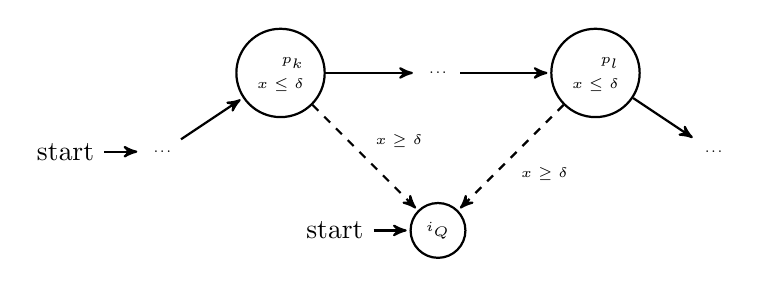
\begin{tikzpicture}[->,>=stealth',shorten >=1pt,auto,node distance=2cm,
  thick,main node/.style={circle,fill=white,draw,font=\sffamily\tiny\bfseries},
  sub node/.style={circle,fill=white,draw,font=\sffamily\tiny\bfseries},
  red node/.style={circle,fill=white,draw,font=\sffamily\tiny\bfseries},
  rec node/.style={rectangle,fill=white,draw,font=\sffamily\tiny\bfseries}]


  \node[main node] (1) [] {$\begin{aligned}p_k\\ x\le \delta\end{aligned}$};
  \node[initial,main node,draw=none] (s1) [left of=1,yshift=-1cm,xshift=0.5cm]{$...$};
  \node[main node,draw=none] (2) [right of=1] {$...$};
  \node[main node] (3) [right of=2] {$\begin{aligned}p_l\\ x\le \delta \end{aligned}$};
  \node[main node,draw=none] (s2) [right of=3,yshift=-1cm,xshift=-0.5cm] {$...$};
  \node[initial,main node] (4) [below of=2]{$i_Q$};


 	\path[every node/.style={font=\sffamily\tiny},dashed]
    (1) edge node {$x\ge \delta$} (4)
    %(2) edge node {$x\ge \delta$} (4)
    (3) edge node {$x\ge \delta$} (4);

    \path[every node/.style={font=\sffamily\tiny}]
    (1) edge node {} (2)
    (2) edge node {} (3)
    (s1) edge node {} (1)
    (3) edge node {} (s2)
    ;

\end{tikzpicture}

\caption{The TA of $P\unrhd_\delta Q$}

\label{interrupt_1}
\end{figure}

Fig.~\ref{interrupt_1} shows the TA of $P \unrhd_\delta Q$ where $p_k$ and $p_l$ are two arbitrary states in $\mcl{F}(P)$.

\item
    Let $\mathcal{F}(P)$ $=(Q_P,\Sigma_P,\mathcal{C}_P,s_P,E_P,I_P,AP_P,L_P,F_P)$ and
    $\mathcal{F}(P_i)$ $=(Q_i,\Sigma_i,\mathcal{C}_i,s_i,E_i,I_i,AP_i,L_i,F_i)$.
    We define $\mathcal{F}(P \unrhd ([]_{i\in I}A_i\to P_i))$
    $=(Q,\Sigma,\mathcal{C},q_0,E,I,AP,L,F)$ as follows:

    \begin{itemize}
    \item $Q=Q_P \cup (\cup_{i\in I} Q_i)$
    \item $\Sigma=\Sigma_P \cup (\cup_{i\in I} \Sigma_i)$
    \item $\mathcal{C}=\mcl{C}_P \cup \mcl{C}_Q \cup \{x\}$
    \item $q_0=i_P$ where $i_P$ is the initial state of $\mathcal{F}(P)$
    \item $AP=AP_P \cup \cup_{i\in I} (AP_{i} \cup \{m_i*\})$
    \item $L=L_P \cup (\cup_{i\in I} L_i)$
    \item $F=\cup_{i\in I} F_i$
        \item $I=I_P \cup (\cup_{i\in I} I_i)$
        \item $E=E_P \cup (\cup_{i\in I} E_i)$ $\cup $ $\{\langle q,\{m_i*\},x==t_{A_i},\{y\},q^\prime \rangle\ |\ $ $q\in Q_P\wedge \exists l_{A_i}\in L(q) \wedge q^\prime=i_{P_i}\}$ where $m_i*$ is either $m_i!$ or $m_i?$ depending on  the type of action $A_i$ ($\bff{Send}$ or $\bff{Get}$). $l_{A_i}$ and $t_{A_i}$ are the start time and location of action $A_i$.
    \end{itemize}

\begin{figure}[htp]
\centering
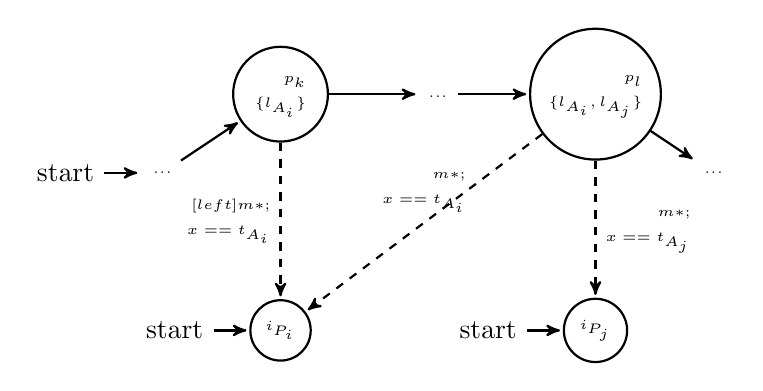
\begin{tikzpicture}[->,>=stealth',shorten >=1pt,auto,node distance=2cm,
  thick,main node/.style={circle,fill=white,draw,font=\sffamily\tiny\bfseries},
  sub node/.style={circle,fill=white,draw,font=\sffamily\tiny\bfseries},
  red node/.style={circle,fill=white,draw,font=\sffamily\tiny\bfseries},
  rec node/.style={rectangle,fill=white,draw,font=\sffamily\tiny\bfseries}]

  \node[main node] (1) [] {$\begin{aligned}p_k\\ \{l_{A_i}\}\end{aligned}$};
  \node [initial,main node,draw=none] (s1) [left of=1,yshift=-1cm,xshift=0.5cm] {$...$};
  \node[rec node] (2) [right of=1,draw=none] {$\begin{aligned}...\end{aligned}$};
  \node[main node] (3) [right of=2]{$\begin{aligned}p_l\\ \{l_{A_i}, l_{A_j}\}\end{aligned}$};
  \node[initial,main node] (4) [below of=1,yshift=-1cm]{$i_{P_i}$};
  \node[initial,main node] (5) [below of =3,yshift=-1cm] {$i_{P_j}$};
    \node [main node,draw=none,right of=3,yshift=-1cm,xshift=-0.5cm] (s2) {$...$};
 	\path[every node/.style={font=\sffamily\tiny},dashed]
    (1) edge node [left]{$\begin{aligned}[left]m*;\\ x==t_{A_i}\end{aligned}$} (4)
    %(2) edge node {$\begin{aligned}m*\\ x==t_{A_i}+\tau(A_i)\end{aligned}$} (4)
    (3) edge node [above]{$\begin{aligned}m*;\\ x==t_{A_i}\end{aligned}$} (4)
    (3) edge node {$\begin{aligned}m*;\\ x==t_{A_j}\end{aligned}$} (5);
    \path[every node/.style={font=\sffamily\tiny}]
    (1) edge node {} (2)
    (2) edge node {} (3)
    (s1) edge node {} (1)
    (3) edge node {} (s2)
    ;

\end{tikzpicture}

\caption{The TA of $P \unrhd ([]_{i\in I}A_i\to P_i)$}
\label{interrupt_2}
\end{figure}

Fig.~\ref{interrupt_2} shows the combination procedure of $P \unrhd ([]_{i\in I}A_i\to P_i)$, where $p_k$ and $p_l$ are two arbitrary states in $\mcl{F}(P)$. $i_{P_i}$, $i_{P_j}$ are the initial states of any $P_i$ and $P_j$ respectively.
From this figure we see that only when location $l_{A_i}$ exists in any state (e.g. $p_l$) of $\mcl{F}(P)$, a transition from $p_l$ to $i_{P_i}$ is built (dashed arrow) for any $i\in I$.

\end{enumerate}


\label{def_stec_to_ta}
\end{mydef}

\begin{mytheo}
The function $\mathcal{F}:\mathbb{P}_{STeC} \rightarrow \mathbb{M}_{TA}$ defined in Definition \rNUM{4}.6 is well defined, and it satisfies $$dom(\mathcal{F})=\mathbb{P}_{STeC}$$
\end{mytheo}
\begin{proof}
It is obvious according to the definition of $\mathcal{F}$.
\end{proof}

\subsection{Simplification of Encoded TA From STeC}
Last section gives a formal definition of the translation from STeC to TA, alert readers may have noticed that in Def.~\ref{def_stec_to_ta} the encoded TA may contain some redundant transitions when rule $\romannumeral5$, $\romannumeral6$ and $\romannumeral7$ are applied during the encoding. For example, when using 'STeC-Sequence' operator (rule $\romannumeral5$) to compose $\mcl{F}(P)$ and $\mcl{F}(Q)$ (where $\mcl{F}(P)$ and $\mcl{F}(Q)$ are two encoded TAs of $P$ and $Q$ respectively), new transitions from final states of $\mcl{F}(P)$ to the inital state of $\mcl{F}(Q)$ (see Fig.~\ref{pseqq}) are added in the new composed TA. Such transitions are redundant since after state $f_P$ is reached, the transition from it to $i_Q$ is immediately fired. The simplification is to removing all redundant transitions in TA.

We firstly give a formal definition of redundant transitions, then give a formal definition of quotient set of states under a function. At last we give the definition of simplification of TAs.

\begin{mydef}
\label{redntfunc}

Let $A$ $=$ $(Q,\Sigma,\mathcal{C},q_0,E,I,AP,L,F)$ be a given Timed Automata. Define $R_A \subseteq E$ as the set of reductant transitions in $A$, where:

\begin{center}
$R_A$ $=$ $\{\langle q,A,g,Y,q^\prime\rangle\ |\ $
$A=\emptyset$

$\wedge$

$\exists y$ $(y\in \mcl{C} \wedge g = y==0 \wedge I(q)\models y\le0 \wedge y\in Y)$

$\wedge$

$\langle q,A,g,Y,q^\prime\rangle \in E$
$\}$.
\end{center}

'$\models$' means 'satisfy' that is defined in a natural way shown in Section \uppercase\expandafter{\romannumeral2}. For example, $y\le0 \models y\le2$, $x\le0 \wedge y\le0 \models y\le 0$.



\end{mydef}

\begin{mydef}
Let $Q$ be any set of states of some TA, $\backsim_R \subseteq Q\times Q$ is a relation on $Q$, then $Q / \backsim_R$ is a quotient set of $Q$ on relation $\backsim_R$ that satisfies:

\begin{center}
    $Q / \backsim_R$ $=$ $\{[q]\ |\ q\in Q\}$
\end{center}

where $\backsim_R$ is a equivalence relation.
$[q] = \{p\ |\ \langle p, q\rangle \in \backsim_R\}$ is the equivalence class of $q$.

\end{mydef}

\begin{mydef}
\label{simTA}
    Given a TA $A$ $=$ $(Q,\Sigma,\mathcal{C},q_0,E,I,AP,L,F)$, define the simplified TA of $A$ as $\bff{Sim}(A)$ $=$ $(Q^\prime,\Sigma^\prime,\mathcal{C}^\prime,q_0^\prime,E^\prime,I^\prime,AP^\prime,L^\prime,F^\prime)$. It satisfies:

\begin{itemize}
    \item $Q^\prime=Q / \backsim_R$, where $\backsim_R \subseteq Q\times Q$ is a relation defined as:
    \begin{center}
        $\backsim_R = \{ \langle p, q\rangle\ |\ $
        $\exists A \exists g \exists Y (\langle p, A, g, Y, q\rangle \in R_A$
        $\vee$
        $\langle q, A, g, Y, p\rangle \in R_A)$
        $\}$ $\cup\ \{\langle p, p\rangle\ |\ p\in Q\}$
    \end{center}

    Easy to see that $R$ is a equivalence relation.

    \item $\Sigma^\prime =\Sigma$
    \item $\mcl{C}^\prime = \mcl{C}$
    \item $q_0^\prime = [q_0]$
    \item $E^\prime = \{\langle [p], A, g, Y, [q]\rangle\ |\ \langle p, A, g, Y, q\rangle \in E\}$
    \item $I^\prime$ is defined as:

    \begin{center}
        $I^\prime([p]) = \bigwedge_{q\backsim_f p} I(q)$.
    \end{center}

    \item $AP^\prime = AP$
    \item $L^\prime$ is defined as:

    \begin{center}
        $L^\prime([p]) = \bigcup_{q\backsim_f p} L(q)$.
    \end{center}

    \item $F^\prime = F / \backsim_R$

\end{itemize}

\end{mydef}

Informally, Def.~\ref{simTA} just 'merge' the states among which reductant transitions exists to make a TA more simpler.

\ifx
\subsection{Using CCSL as a specification language of STeC}
\fi

\ifx
\section{Bisimilarity---Relationship between STeC and Transformed TA}
In the last section we see that a homomorphism is built for the transformation from STeC to timed automata. In this section we proof that any STeC formula and its transformed timed automata are bisimilar, which means that the expressive power of any transformed TA is as strong as that of the corresponding STeC formula (In other words, for whatever systems STeC can model, TA also can) under some reasonable sense.

Regularly, 'bisimulation' is considered as a partial order relation between two 'processes' in one type of process algebra language or two 'states' in one type of transition system language. The problem is that we are trying to analyse the bisimilarity between a process algebra language---STeC and a type of transition system language---Timed Automata. One solution is that we trivially embedded both STeC and TA into a type of transition system, and consider the simulation property in it under some reasonable sense. As a beginning, Def.~\ref{def_tran} give a definition of 'transition system' where we mimic a type of definition in process algebra book but here the type of set of actions is emphasized.

\begin{mydef}
A transition system(or process graph) is a tuple $(\mathbb{S},\mathbf{Act},\Longrightarrow)$, where $\mathbb{S}$ is a set of states, $\mathbf{Act}$ is a set of actions, and $\Longrightarrow \subseteq \mathbb{S} \times \mathbf{Act} \times \mathbb{S}$ is a transition relation.

\label{def_tran}
\end{mydef}

\begin{mydef}
Function $\xi : \mathbb{P}_{STeC} \to \mathbb{S}$ is a bijection which maps each STeC formula to a state in $\mathbb{S}$. Simply, write $\xi(P)$ as $P^{\xi}$.

Define a closure $Cl : \mathbb{P}_{STeC} \to 2^{\mathbb{P}_{STeC}}$ in STeC. Briefly, for any $P \in \mathbb{P}_{STeC}$, $Cl(P)$ is a set of all of its subprocesses.

We embedded each STeC formula into a transition system $(\mathbb{S},\mathbb{E}_{STeC},\Longrightarrow)$ with $\mathbb{E}_{STeC}$ be its action set by defining a function $T_{STeC} : \mathbb{P}_{STeC} \to \{(\mathbb{S},\mathbb{E}_{STeC},\Longrightarrow) | \mathbb{S} \subseteq \xi(\mathbb{P}_{STeC})\}$. For any $P \in \mathbb{P}_{STeC}$, $T_{STeC}(P)$ is a transition system $(\xi(Cl(P)),\mathbf{Words}(P),\Longrightarrow)$ which satisfies:

Set 'a' be any atomic action and $e_a=\langle a, l_a, t_a, \delta_a \rangle$ is its corresponding word in $\mathbf{Words}(P)$, and $P_1, Q_1 \in Cl(P)$, then $\Longrightarrow(P_{1}^{\xi},e_a,Q_1^{\xi})$ iff $P_1=a \to Q_1$ holds. Often, write $\Longrightarrow(P_1^{\xi},e_a,Q_1^{\xi})$ as $P_1^{\xi} \overset{e_a}{\Longrightarrow} Q_1^{\xi}$.

\label{def_tran_stec}
\end{mydef}

Def.~\ref{def_tran_stec} says that each STeC formula is equivalent to a transition system defined in Def.~\ref{def_tran} in the sense of bijection mapping $\xi$.

Embedding a timed automata into a transition system defined in Def.~\ref{def_ta_tran} is quite trivial.

\begin{mydef}
\label{def_ta_tran}
Use $Inv_A$ to represent the set of all invariants in timed automata $A$.

Function $\eta : \mathbb{M}_{TA} \times \{Inv_A | A \in \mathbb{M}_{TA}\} \to \mathbb{S}$ maps each state and its invariant function in TA into a state in $\mathbb{S}$.
For any $\langle s, I(s)\rangle$ in a timed automata $A \in \mathbb{M}_{TA}$, simply write $\eta(\langle s, I_A(s)\rangle)$ as $s_A^{\eta}$. $\eta$ is a bijection.

Trivially, any timed automata $A \in \mathbb{M}_{TA}$ can be embedded into a transition system $(\mathbb{S}, E, \Longrightarrow)$ where $E$ is any transition relation set. Define a function $T_{TA} : \mathbb{TA} \to \{(\mathbb{S}, E_A, \Longrightarrow) | \mathbb{S} \subseteq \eta(A \times Inv_A)\}$, for any $A=(Q_A,\Sigma_A,\mathcal{C}_A,q_0^A,E_A,I_A,AP_A,L_A,F_A) \in \mathbb{M}_{TA}$, it satisfies:

For any $s, t \in Q_A$, we have $\Longrightarrow(s_A^{\eta}, e, t_A^{\eta})$ iff $\exists e \in E_A$ from $s$ to $t$. Often we denote $\Longrightarrow(s_A^{\eta}, e, t_A^{\eta})$ as $s_A^{\eta} \overset{e}{\Longrightarrow} t_A^{\eta}$.

\end{mydef}

It is obvious that each timed automata is equivalent to a transition system defined in Def.~\ref{def_tran} in the sense of a bijection mapping $\eta$.

Def.~\ref{def_tran_stec}, Def.~\ref{def_ta_tran} say that
for any $P \in \mathbb{P}_{STeC}$ and $A \in \mathbb{M}_{TA}$, $T_{STeC}(P)$ is a equivalent transition system $(\xi(Cl(P)),\mathbf{Words}(P),\Longrightarrow)$ in the sense of bijection $\xi$. $T_{TA}(A)$ is a equivalent transition system $(\eta(Q_A),E_A,\Longrightarrow)$ in the sense of bijection $\eta$.


With Def.~\ref{def_tran_stec} and Def.~\ref{def_ta_tran}, we convert both STeC and TA into their equivalent same 'type' of transition system. Next we proof that under some reasonable sense, any STeC formula and its transformed TA are bisimilar, which is the main result in this section.

\begin{mydef}
Let $\mathbf{Act_1}$, $\mathbf{Act_2}$ be two different type of actions. There is a function $f : \mathbf{Act_2} \to \mathbf{Act_1}$ between these two sets. Given two transition systems: $S_1=(\mathbb{S}_1, \mathbf{Act_1}, \Longrightarrow)$ and $S_2=(\mathbb{S}_2,\mathbf{Act_2},\Longrightarrow)$, we say that $S_1$ can simulate $S_2$ in the sense of $f$, denoted as $S_2 \ll_{f} S_1$, iff for any state $q \in \mathbb{S}_2$
there exists a state $p \in \mathbb{S}_1$ such that $q \ll_{f} p$.

Define $q \ll_{f} p$ as follows:

for any action $a \in \mathbf{Act_1}$, if $q \overset{a}{\Longrightarrow} q^\prime$ then $p \overset{f(a)}{\Longrightarrow} p^\prime$ holds where $f(a) \in \mathbf{Act_2}$, and more $q^\prime \ll_{f} p^\prime$ holds.

If $S_1 \ll_{f} S_2$ and $S_2 \ll_{f} S_1$ hold, $S_1$ and $S_2$ are bisimilar, namely $S_1 \approx_{f} S_2$, called that $S_1$ and $S_2$ are bisimilar in the sense of $f$, and $f$ is a bijection. Trivially, we can proof that bisimulation $\approx_{f}$ is an equivalent relation.
\end{mydef}

We need this lemma before the final proof.

\begin{lemma}
Given any $P \in \mathbb{P}_{STeC}$, we can generate a bijection $\mathcal{F_*} : \mathbf{Words}(P) \to E_{\mathcal{F}(P)}$ from the homomorphism $\mathcal{F}$.
\begin{proof}
.........................................................
\end{proof}
\end{lemma}

\begin{mytheo}
\label{bisim}
For any $P \in \mathbb{P}_{STeC}$, $\mathcal{F}(P)$ is its corresponding timed automata transformed using Def.~\ref{def_stec_to_ta}. And $T_{STeC}(P)=(\xi(Cl(P)),\mathbf{Words}(P),\Longrightarrow)$, $T_{TA}(\mathcal{F}(P)) = (\eta(Q_{\mathcal{F}(P)}),E_{\mathcal{F}(P)},\Longrightarrow)$ are their corresponding equivalent transition system which is defined according to Def.~\ref{def_tran}, ~\ref{def_tran_stec} and ~\ref{def_ta_tran}. Then we can generate a bijection $\mathcal{F}_*: \mathbf{Words}(P) \to E_{\mathcal{F}(P)}$ from $\mathcal{F}$ such that in the sense of which $T_{TA}(\mathcal{F}(P))$ and $T_{STeC}(P)$ are $\mathcal{F_*}$-bisimilar, denoted as
$$T_{STeC}(P) \approx_{F_*} T_{TA}(\mathcal{F}(P))$$.

\begin{proof}
...................................................
\end{proof}

\end{mytheo}

We can imagine the function '$\mathcal{F}_*$' as a 'translation' from STeC words to TA transitions. Theo.~\ref{bisim} tells us in fact STeC formula and its transformed TA share the same 'execution-branching' tree structure except for the 'actions', but we can translate each STeC 'action' to its corresponding TA 'action'(here the 'action' is what we define in Def.~\ref{def_tran}, readers should differ it from the action in STeC or TA. An action in STeC is just an alphabet of an atomic process.), and such a translation is a one-to-one mapping(bijection). The result indicates that if we admit such an bijective 'translation'(in other word, think such a 'translation' is reasonable or acceptable), then in such sense we can say they are bisimilar, which means such a transformation $\mathcal{F}$ from STeC to TA is reasonable.
\fi

\section{An Example of ITS---Railroad Crossing System}
In this section, we gives an ITS example showing how to use our proposed verification framework introduced in Section \uppercase\expandafter{\romannumeral3}. As Fig.~\ref{RCP} shows, a 'Railroad Crossing System' is an autonomous ITS system where a behaviour is required to be fired at right location and time. In the next few subsections, we will show how to use STeC to model this system and CCSL to specify some safety properties. And we gives a result of encoded TAs of STeC-model of this system by applying Def.~\ref{def_stec_to_ta} and a result of corresponding UPPAAL TAs generated by our implemented automatic encoding tool.

\ifx
Modeling and verifying Intelligent Transportation Systems using the proposed new verification framework is the main goal of our research. We want to design neater, nicer and more importantly easier-understandable modeling language for engineers to use at design-level of the development of Intelligent Transportation Systems without losing any expressive power when comparing the old modeling languages like timed CSP, and transform it into 'complex' languages such as TA in order to do verification. On the other hand, automatic tools should be implemented when people come up with a new formal language, only then it possibly becomes a powerful tool widely used in industry. In this section, we consider a classical example called 'railroad crossing system' shown in Fig.~\ref{RCP}.
In the next few subsections we use this example to show how to use STeC and CCSL as our new verification techniques to model behaviours and specify properties of intelligent transportation systems.
\fi

In 'Railroad Crossing System' shown in Fig.~\ref{RCP}, there are two agents: a train and a gate. The railroad lies in the east-west direction and the road lies in the south-north direction.
The scenario of the system is stated as follows:

\begin{itemize}
    \item When there is no train approaching the gate, gate should be kept open so vehicles can pass the crossing.
    \item When a train approaches, it sends message 'Approach' to the gate informing that it is approaching. The gate receives the message and the program of gate tells whether to close the gate or keep it open according to the traffic condition of the crossing:
        \begin{enumerate}[1.]
            \item if the gate cannot be closed, the gate sends message 'NonClose' back to the train informing that the train should be stopped. And wait until it can.
            \item if the gate can be closed, sends message 'Close' back to the train telling the train can pass safely.

        \end{enumerate}
    \item The train receives message from gate:
        \begin{enumerate}[1.]
            \item if getting message 'NonClose', it should be stopped and wait message 'Close' for a safe passing.
            \item if getting message 'Close', it can safely pass the crossing.
        \end{enumerate}

    \item After the train safely pass the crossing, it sends message 'Pass' to the gate, the gate should be opened.

\end{itemize}

We use 'Lapp','Lpass','Lstop' and 'Lleav' to notate the locations at which the train arrive at different time, and
'Open', 'Closed' to notate the locations(states) at which the gate be at different time. The next we use STeC to model the scenario described above (as a comparison, in \cite{roscoe83} a similar 'train' system is described using CSP).

\ifx
The railroad lies in the east-west direction and the road lies in the south-north direction.
When no train pass by, gate is open so the vehicles are allowed pass the cross. When a train comes,
the train communicate with the gate to avoid collision on the crossing: it sends the gate a message 'Approach' to inform that it is approaching. The gate receive the message and make a judgement according to the traffic condition on the road, and then sends the message back to the train which in turn makes a judgement on what is going to do next according to this. If the gate is allowed to close, then the gate sends a message 'Close' back to the train, then the train can pass the gate, or the gate sends 'NonClose' back to the gate, then the gate have to stop and wait the gate open. After the train passes, the train sends a message 'Leav' to the gate, the latter should be opened again so that vehicles can pass again. It is a real-time system in which the time and location involves. In Fig.~\ref{RCP}, we can see that 'Lapp','Lpass','Lstop' and 'Lleav' are locations at which train do certain action at certain time. We call such a constraint special-temporal specification and we use STeC as the 'right' language to describe such type of specifications (As a comparison, in \cite{roscoe83} a similar 'train' system is described using CSP).
\fi

\subsection{Modeling ITS Using STeC}
We firstly describe train agent and gate agent agent using STeC, and then compose them using parallel operator '$||$' shown before.

\begin{figure}[htp]
\centering
\includegraphics[width=2.5in]{graph/Train_Gate.png}
\caption{Railroad Crossing System}
\label{RCP}
\end{figure}


%\begin{figure}[htp]
%\centering
%\includegraphics[width=2.5in]{graph/RCP.PNG}
%\caption{Railroad Crossing Problem}
%\label{RCP}
%\end{figure}

\subsubsection{Train Agent}Let $P_{Train}$ be the name of train agent process and $P_{Gate}$ be the name of gate agent.  Let $A_{Train}$, $A_{Gate}$ be the corresponding encoded TA. Then we have:

$$P_{Train}\ =\ Run(\infty); (Send_{(Lapp,t,G)}(Appr) \parallel $$
$$Approach_{(Lapp,t)}(\Gamma)) ;$$
$$\left\{ \begin{array}{l l}
Get_{(Lpass,t+\Gamma,G)}(Cross) \to (Pass_{(Lpass,t+\Gamma)}(\triangle);\\
\hspace{1cm}(Send_{(Lleav,t+\Gamma+\triangle,G)}(Lleav) ; P_{Train})) \\
\talloblong \\
Get_{(Lpass,t+\Gamma,G)}(Noncross) \to (Stop_{(Lpass,t+\Gamma)}(\Upsilon);\\
Wait_{(Lstop,t+\Gamma+\Upsilon,G)}(Cross);Pass_{(Lstop,t\prime+\Omega,G)}(\Omega);\\
\hspace{1cm} (Send_{(Lleav,t \prime+\Omega,G)}(Lleav) ; P_{Train}))
\end{array}
\right\}$$

The train approaches the crossing at 'Lappr, it sends message 'Appr' to the gate, informing that there is a train coming. After $\Gamma$ time the train tries to get a message from the gate. If it gets message 'Cross', the gate has been closed and it can pass safely. If it gets the "NonCross" message, then it stops and waits for the gate to be closed. After the train has passed, it sends message 'Leave' to inform the gate.

Applying Def.\ref{def_stec_to_ta}, we can use the function $\mathcal{F}(P_{Train})$ to transform the model
$P_{Train}$ into a TA inductively:
$$
\mathcal{F}(P_{Train})=\mathcal{F}(Run(\infty);P_{Train}^\prime)$$
$$=\mathcal{F}(Run(\infty)) \diamond_{STeC}
\mathcal{F}(P_{Train}^\prime)
$$
$$
=A_{Run(\infty)} \diamond_{STeC} \mathcal{F}(\
(Send_{(Lapp,t,G)}(Appr) \parallel $$
$$Approach_{(Laap,t)}(\Gamma)) ;$$
$$
\hspace{1cm}\left\{ \begin{array}{ll}
Get_{(Lpass,t+\Gamma,G)}(Cross) \to (Pass_{(Lpass,t+\Gamma)}(\triangle);\\
\hspace{1cm}(Send_{(Lleav,t+\Gamma+\triangle,G)}(Lleav) ; P_{Train})) \\
\talloblong \\
Get_{(Lpass,t+\Gamma,G)}(Noncross) \to (Stop_{(Lpass,t+\Gamma)}(\Upsilon);\\
Wait_{(Lstop,t+\Gamma+\Upsilon,G)}(Cross);Pass_{(Lstop,t\prime+\Omega,G)}(\Omega);\\
\hspace{1cm} (Send_{(Lleav,t \prime+\Omega,G)}(Lleav) ; P_{Train}))\\
\end{array}\right.
$$
$$
)
$$
$$
=A_{Run(\infty)} \diamond_{STeC} \mathcal{F}(P_1; P_2)=A_{Run(\infty)} \diamond_{STeC} \mathcal{F}(P_1; P_2)
$$
$$
=A_{Run(\infty)} \diamond_{STeC} \mathcal{F}(P_1) \diamond_{STeC} \mathcal{F}(P_2)=......=A_{Train}.
$$

where $P_1=Send_{(Lapp,t,G)}(Appr) \parallel Approach_{(Laap,t)}(\Gamma)$ and

$$P_2=\left\{ \begin{array}{ll}
Get_{(Lpass,t+\Gamma,G)}(Cross) \to (Pass_{(Lpass,t+\Gamma)}(\triangle);\\
\hspace{1cm}(Send_{(Lleav,t+\Gamma+\triangle,G)}(Leave) ; P_{Train})) \\
\talloblong \\
Get_{(Lpass,t+\Gamma,G)}(Noncross) \to (Stop_{(Lpass,t+\Gamma)}(\Upsilon);\\
Wait_{(Lstop,t+\Gamma+\Upsilon,G)}(Cross);Pass_{(Lstop,t\prime+\Omega,G)}(\Omega);\\
\hspace{1cm} (Send_{(Leave,t \prime+\Omega,G)}(Lleav) ; P_{Train}))\\
\end{array}\right.
$$

Finally we simplify $A_{Train}$ by applying Def.~\ref{simTA}, and we get $\bff{Sim}(A_{Train})$ as the TA of the process $P_{Train}$. The result of $\bff{Sim}(A_{Train})$ is shown in the following figure(Fig.~\ref{TAgent}).

\begin{figure}[htp]
\centering
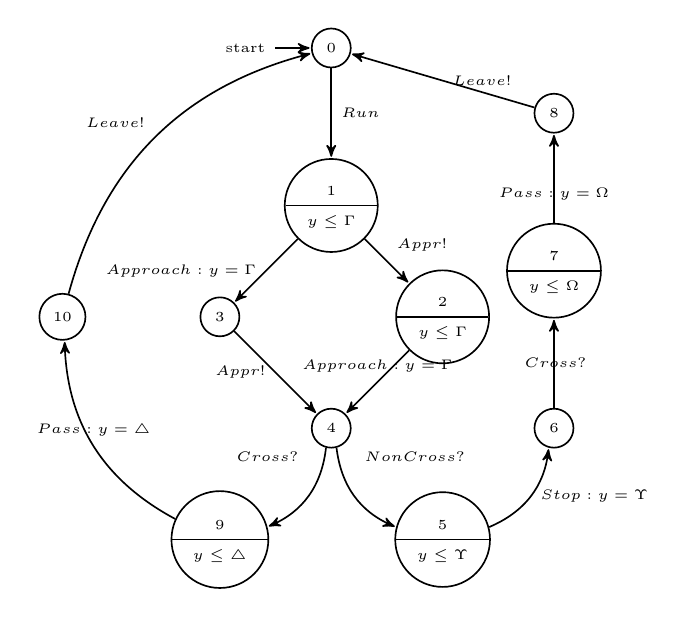
\begin{tikzpicture}[->,>=stealth',shorten >=0.5pt,auto,node distance=2.0cm,
                    semithick]
  \tikzstyle{every state}=[text=black,font=\tiny,minimum size=0pt]
  \tikzstyle{every node}=[font=\tiny,minimum size=0pt]
\node [initial,state] (0) {$0$};
\node [state with output] [below of=0] (9) {$1$ \nodepart{lower} $y \le \Gamma$};
\node [state with output] [below right of=9](1) {$2$ \nodepart{lower} $y \le \Gamma$};
\node [state] [below left of=9] (10) {$3$};
\node [state] (2) [below right of=10] {$4$};
\node [state with output] (3) [below left of=2] {$9$ \nodepart{lower} $y \le \triangle$};
\node [state] (4) [left of=10] {$10$ \nodepart{lower}};
\node [state with output] (5) [below right of=2] {$5$ \nodepart{lower} $y \le \Upsilon $};
\node [state] (6) [above right of =5] {$6$};
\node [state with output] (7) [above of=6] {$7$ \nodepart{lower} $y \le \Omega$};
\node [state] (8) [above of=7] {$8$};

\path (0) edge node {$Run$} (9)
	  (9) edge node [left] {$Approa
      ch:y=\Gamma$} (10)
      (10) edge node [left] {$Appr!$} (2)
      (9) edge node {$Appr!$}    (1)
      (1) edge node [above]{$Approa
      ch:y=\Gamma$} (2)
      (2) edge [bend left] node [left,yshift=0.5cm]{$Cross?$} (3)
          edge [bend right] node [right,yshift=0.5cm]{$NonCross?$} (5)
      (3) edge [bend left] node [above] {$Pass:y=\triangle$} (4)
      (4) edge [bend left] node {$Leave!$} (0)
      (5) edge [bend right] node [right] {$Stop:y=\Upsilon$} (6)
      (6) edge node [right,xshift=-0.5cm] {$Cross?$} (7)
      (7) edge node [below] {$Pass:y=\Omega$} (8)
      (8) edge node [right] {$Leave!$} (0);

	\end{tikzpicture}
\caption{The Encoded TA (simplified) From Train Agent Process in STeC}
\label{TAgent}
\end{figure}

Assume that $A_{Train}=(Q,\Sigma,\mathcal{C},q_0,E,I,AP,L,F)$ is the corresponding TA translated from STeC, the following gives some explanations of $A_{Train}$:
\begin{itemize}
\item
$Q=\{0,1,2,3,4,5,6,7,8,9,10\}$ is the set of locations of TA.

\item
$\Sigma=\{Run,Appr!,Cross?,Approach,Pass,Noncross?$

$,Stop,Cross?,Leave!\}$ corresponds to the actions of $P_{Train}$.

\item
$\mathcal{C}=\{x,y\}$. Two clocks, one for recording total time from the beginning and one for recording the delay of actions in STeC.

\item
$E \subseteq Q \times 2^\Sigma \times G(\mathcal{C}) \times 2^{\mathcal{C}} \times Q$ is the set of transition relation of $A_{Train}$. For example, the transition from state $1$ to state $3$ is a tuple: $\langle 1,\{Approach\},\{y=\Gamma\},\{y\},3\rangle$, where '$Approach$' is the action name, '$y=\Gamma$' is the guard condition, '$y$' is the clock set to be zero after transition is fired.

\item
$q_{0}=0$ is the initial state.

\item
$I:Q \to G(\mathcal{C})$ maps each state to a guard expression. For example, $I(1)=y\le \Gamma$, so $\Gamma$ time after being in state $1$, the transition is forced to be fired.

\ifx
we can only stay
at most $5$ units of time and after that, any transition which satisfies the guard condition must happen, or (if no such
transitions exists) no further progress is possible. In some states, one transition
must happen when the state no longer satisfy its invariant, for example, state $9$ and state $10$. Since the
invariant is $y \le \triangle$, so the action $Pass$ is executed immediately when the clock $y$ equals $\triangle$.
\fi

\item
$L:Q \to 2^{AP}$ is the labelling function.	The location in STeC is the atomic proposition in TA. For example, we have
$L(10)=\{Lleav\}$, $L(1)=\{Lapp\}$,$L(4)=\{Lpass\}$, $L(0)=\emptyset $, etc.

\end{itemize}
\subsubsection{Gate Agent}Following the same procedure, we can get the encoded $A_{Gate}$ from $P_{Gate}$.
$$P_{Gate}\ =\ (Get_{(Open,t,G)}(Appr) \to Closing_{(Open,t+\theta_0)}(\Pi));$$
$$\left\{ \begin{array}{l l}
(Closed_{(Closed,t+\theta_0+\Pi)}(1) ; \\
Send_{(Closed,t+\theta_1,G)}(Cross)
;
(Get_{(Closed,t+\theta_2)}(Leav) \\
\to Opening_{(Closed,t+\theta_2)}(\zeta))));P_{Gate}\\
\talloblong \\
(Unclosed_{(Unclosed,t+\theta_0+\Pi)}(0) ; \\
(Send_{(Unclosed,t+\theta_0+\Pi,G)}(NonCross) \parallel \\
Clossing_{(Unclosed,t+\theta_0+\Pi)}(\pi)) \\
;(Closed_{(Closed,t+\theta3)}(0) \parallel
(Send_{(Closed,t+\theta_3,G)}(\\
Cross));
(Get_{(Closed,t^\prime+\Omega,G)}(Leav) \\
\to Opening_{(Closed,t^\prime+\theta_4)}(\zeta)
);P_{Gate}\\
\end{array}
\right\}$$

For the gate agent, it starts with waiting for message 'Appr'. Then the program of gate decides whether close the gate or not. If it is successfully closed, it sends message 'Cross', then waits for message 'Leave' from train to be safe to be opened again. If it is not closed, sends message 'NonClose'.

\ifx
For the agent Gate, it begins with the location "Open" and wait for the message "Appr" sent by train. Then the gate tries to close the gate. If the gate is successfully closed, then it send "Cross" message to train. Then keep listening the train's message until message "Leav" is received. Open the gate and then again keep listenning. If the gate is not closed. Send "NonCross" message to train to stop the train and try to close again. Send the "Cross" message to train if it is successfully closed and reopen it after receiving "Leav".
\fi

We can get the simplified version of $A_{Gate}$ as $\bff{Sim}(A_{Gate})$, which is shown in Fig.~\ref{TAGate} :

\begin{figure}[htp]
\centering
\begin{tikzpicture}[->,>=stealth',shorten >=1pt,auto,node distance=2cm,
                    semithick]
  \tikzstyle{every state}=[text=black,font=\tiny,minimum size=0pt]
  \tikzstyle{every node}=[font=\tiny,minimum size=0pt]
\node [initial,state] (0) {$0$};
\node [state with output] [below of=0] (1) {$1$ \nodepart{lower} $y \le \Pi$};
\node [state] [below of=1](2) {$2$};
%\node [state with output] (3) [below left of=2] {$3$ \nodepart{lower} $y \le 1$};
\node [state with output] (4) [above left of=3] {$3$ \nodepart{lower} $y \le 0$};
\node [state] (5) [above of=4] {$4$};
\node [state with output] (6) [above of=5] {$5$ \nodepart{lower} $y \le \zeta $};

%\node [state with output] (7) [right of=2] {$7$ \nodepart{lower} $y\le \pi$};
\node [state with output] (8) [below right of=2,xshift=1cm] {$6$ \nodepart{lower} $y \le \pi$};
\node [state] (12) [above of=8] {$10$};
\node [state] (9) [above of=12] {$7$ \nodepart{lower} };
\node [state] (10) [above of=9] {$8$ };
\node [state with output] (11) [above of=10] {$9$ \nodepart{lower} $y \le \zeta$};

\path (0) edge node [left]{$Appr?$} (1)
      (1) edge node [left]{$Closing:y = \Pi$}(2)
      %(2) edge node [left] {} (3)
      %(2) edge node {} (7)

      (2) edge node {$Close:y=1:\{y\}$} (4)
      (4) edge node {$Cross!:\{y\}$} (5)
      (5) edge node {$Leav?:\{y\}$} (6)
      (6) edge [bend left] node [above] {$Opening:y=\zeta$} (0)

      (2) edge node {$NonCross!$} (8)
      (8.east) edge [bend right] node [above] {$Closing:y=\pi$} (9.east)
      (9) edge node {$Close!$} (10)
      (10) edge node {$Leav?$} (11)
      (11) edge [bend right] node [above]{$Opening:y=\zeta$} (0)

    (2) edge [] node [above]{$Closing:y=\pi$} (12)
    (12) edge node [above] {$NonCross!$} (9);
	\end{tikzpicture}
\caption{The Encoded TA (simplified) From Gate Agent Process in STeC}
\label{TAGate}
\end{figure}

\subsubsection{Railroad Crossing System}The railroad crossing system as a whole is defined as $$P_{Sys}=P_{Train} \parallel P_{Gate}$$

The corresponding TA is as follows:
$$
A_{Sys}=\mathcal{F}(P_{Sys})=\mathcal{F}(P_{Train} \parallel P_{Gate})=A_{Train} \otimes_{STeC} A_{Gate}
$$

\subsection{Modeling System in Practice Using STeC}
We implemented a tool that takes STeC text as input and output Uppaal Timed Automatas (visit www.uppaal.org for more information about UPPAAL). The next we give the results of encoded TAs of this system by applying our implemented tool. We omit the details of architecture of this tool which is beyond the theme of this paper. Since the implemented encoding algorithm is slightly different from Def.\ref{def_stec_to_ta}. So the result of encoded TAs(shown in Fig.~\ref{uppaalta} and Fig.~\ref{uppaalta2}) are subtle different from the encoded TAs in Fig.~\ref{TAgent} and Fig.~\ref{TAGate} which are the direct results from Def.\ref{def_stec_to_ta}.

\ifx
We only use this example to show how to describe the 'Train Agent' in the 'Railroad Crossing System' using STeC code and the result of TA in Uppaal.
\fi

In the following we show the STeC code for the 'Railroad Crossing System'.
Here is the description of the train agent.

\lstset{
basicstyle=\ttfamily\small,
emph={TIME,LOCATION,MESSAGE,Get,Send,CHANNEL,ALPHA,BETA},emphstyle=\textbf
}

\begin{lstlisting}
//Declarations
TIME t=0.	   //time for starting
TIME t_appr=5.	//time spent on approach
TIME t_pass=10.	//time spent on pass
TIME t_stop=8.	//time spent on stop

LOCATION Lpass, Lleav, Lstop, Lapp //location \\
                            of train agent

MESSAGE Cross, Leave, NonCross //messages of \\
                                train agent

CHANNEL Send, Get //communication actions of \\
                    Train agent

ALPHA Pass, Stop, Approach //alpha actions

BETA Run //beta actions

//subprocesses P1 and P2
#define P1 \
  (Get(Lpass)(Cross)->Pass(Lpass)(Lleav,$t_pass)-> \
  Send(Lleav)(Leave))

#define P2 \
  (Get(Lpass)(NonCross)->Stop(Lpass)(Lstop,$t_stop)\
  -> Get(Lstop)(Cross)->Pass(Lstop)(Lleav, $t_pass)\
  -> Send(Lleav)(Leave))

//Train Process
Train=@T(
  Run()();Send(Lapp,$t)(Appr)-> \
  Approach(Lapp)(Lpass,$t_appr)-> \
  (P1 [] P2) -> #T
).

\end{lstlisting}

In the block of STeC code shown above, we firstly give declarations of different components of STeC language like time, location, message or channel. '\textbf{TIME}', '\textbf{LOCATION}' and '\textbf{MESSAGE}' are the key words of declaration of time, location and message respectively. Two channels '\textbf{Send}' and '\textbf{Get}' are synchronization actions of type $A$ in STeC declared by key word '\textbf{CHANNEL}'. '\textbf{ALPHA}' and '\textbf{BETA}' represent the '$\alpha$' and '$\beta$' type of actions that is defined in Section \uppercase\expandafter{\romannumeral2}.

 In the above example, we define $4$ time variables: 't', 't\_appr', 't\_pass' and 't\_stop'. $4$ locations 'Lpass', 'Lleav', 'Lstop' and 'Lapp'. There are three messages for train agent, that is 'Cross', 'Leave' and 'NonCross'. 'Pass', 'Stop' and 'Approach' are the names of '$\alpha$' type of actions. 'Run' is a '$\beta$' action since it does not involve any change of locations. Its 'location' and 'duration' factors being omitted shows that the location and duration of this action are not required.

 Two macro 'P1' and 'P2' are subprocesses. The key word '\#define' has similar meaning as in C++/C. The macro is substituted for its body during the pre-compilation process.

'Train' is the formula of train process.
'@T' is a recursion symbol. It defines a sub formula of 'Train' for which '\#T' is substituted at each of its ocurrences.
For example, after the subprocess '(P1 [] P2)' is fired, then we replace the symbol '\#T' with the sub formula notated by '@T', that is:

\lstset{
basicstyle=\ttfamily\small,
emph={TIME,LOCATION,MESSAGE,Get,Send},emphstyle=\textbf
}

\begin{lstlisting}
  Run()();Send(Lapp,$t)(Appr)->
  Approach(Lapp)($t_appr)-> (P1 [] P2) -> #T
\end{lstlisting}

So the action 'Run()()' should be fired next.


\ifx
in the 'Train process' that is defined next. In 'Train process', we define a process variable named 'Train',
and describe its behaviour as the STeC formulas that we saw in the previous section. '@T' is a recursion symbol.

Here is the description of Gate agent.
\lstset{
basicstyle=\ttfamily\small
}

\begin{lstlisting}

//Gate Agent
t_close=4. //time spent on close
t_open=4. //time spent on open

//Two macros P3 and P4
#define P3 ( \
	Closed(Closed)(1)->Send(Closed)(Cross)->\
        Get(Closed)(Leave) \
	->Opening(Closed)($t_open);#G \
)

#define P4 ( \
	Unclosed(Unclosed)(0)->( \
		Send(Unclosed)(NonCross)|| \
        Closing(Unclosed)($t_close) \
		)-> \
	Send(Closed)(Cross)-> \
        Get(Closed)(Leave)-> \
	Opening(Closed)($t_open);#G \
)

//Gate Process
Gate=@G(
	Get(Open,$t)(Appr)-> \
        Closing(Open)($t_close);
	(P3 [] P4)
).

\end{lstlisting}
\fi

As the result of STeC tool here we just give the corresponding transformed TA for Train Agent drawn with 'graphviz' tool\footnotemark[1]\footnotetext[1]{'graphviz' is a famous open source visualization tool, visit http://www.graphviz.org/ for more information.} (Fig.~\ref{graphvizgate}), where the red node 'Get\_S106' is the initial state and the green node 'F\_211' is the final state. The encoded TA of UPPAAL format is shown in Fig.~\ref{uppaalta} and Fig.~\ref{uppaalta2} in Appendix A.


\begin{figure}[htp]
\centering
\includegraphics[scale=0.25]{graph/Gate_272.png}
\caption{The TA of Gate Agent Drawn Using graphviz tool}
\label{graphvizgate}
\end{figure}

\subsection{Specifying Properties Using CCSL}
As introduced before, we defined CCSL as the specification language in the domain of STeC. Def.~\ref{def_clock_stec} and Der.~\ref{sat} show the details. Next we give an example using CCSL to specify the properties of 'Railroad Crossing System'.

In the 'Railroad Crossing System' introduced above, we find two safety properties that people usually care about:

\vspace{0.5cm}
\centerline{\textbf{Property 1}: When the train passes, the gate must be closed.}

\vspace{0.5cm}
Using CCSL, we have the following expressions:

\vspace{0.5cm}
\centerline{$c_{close} \prec c_{mayPass} \prec c_{open}$;}

\centerline{$c_{close}$ \textbf{Alternate} $c_{open}$;}

\centerline{$c_{pass} \subset c_{mayPass}$;}

\vspace{0.5cm}
'$\prec$' means 'precedence' in CCSL, the first formula says the clock 'close' always ticks before the clock 'mayPass' and the clock 'mayPass' always ticks before the clock 'open'. The second formula says that the clock 'close' and the clock 'open' tick alternately. The third formula says that clock 'pass' is a subclock of the clock 'mayPass', which means that whenever the clock 'pass' ticks, the clock 'mayPass' must tick. Consulting the definition of these operators in CCSL(see the previous section of the introduction of CCSL or for more details, refer to [10]), this CCSL constraint means exactly the Property 1 mentioned above.

 Using Timesquare we have a possible trace satisfying the CCSL constraint shown in Fig.~\ref{sim1}.

\begin{figure}[htp]
\centering
\includegraphics[scale=0.45]{graph/CCSL_1.PNG}
\caption{Simulate result of Property 1}
\label{sim1}
\end{figure}

Considering another property:

\vspace{0.5cm}
\centerline{\textbf{Property 2}: Once the train approaches, }

\centerline{the gate shall close in at most 1 minutes.}

\vspace{0.5cm}
It contains a time expression '1 minutes'. We use the operator '\textbf{DiscretizeBy}' in CCSL to generate a new discrete-time clock $c_{time}$ that ticks every 1 ms based on an '\textbf{IdealClock}'. The expression of \textbf{Property 2} is given as follows:

\vspace{0.5cm}
\centerline{$c_{appr} \prec c_{close} \prec c_{appr\_delay}$;}

\centerline{$c_{appr\_delay} = c_{appr}$ \textbf{delay} $1000$  \textbf{on} $c_{time}$;}

\vspace{0.5cm}
\ifx
 In the second formula, symbol '\$' means 'delay' in CCSL. It says that the clock 'appr\_delay' ticks 1 units of time delay for the clock 'appr'.
 \fi

 $c_{time}$ is a 'discrete-time' clock, it is defined as follows:

 \begin{center}
$c_{time} =$ \textbf{IdealClock} \textbf{DiscretizeBy} $1$ ms
 \end{center}

Let \textbf{IdealClock} $= \langle \mcl{I}_A, \prec, \lambda_A, \mbb{R}^+, \mu_A\rangle$, $c_{time}=\langle \mcl{I}_B, \prec, \lambda_B, \mbb{R}^+, \mu_B\rangle$. Since $\mcl{I}_B$ is discrete, so we set $i^{++}$ be the successor of $i$ for any $i\in \mcl{I}_B$. $P \subseteq \mcl{I}_A \times \mcl{I}_B$ is defines as:

$$P(j,i)=\left\{\begin{array}{ll}
true & \mbox{if $h(i) \prec j \prec h(i^{++})$}\\
\\
false & \mbox{otherwise}\\
\end{array}\right.
$$

where $h : \mcl{I}_B \rightarrow \mcl{I}_A$ is defined as follows:

$(\forall i\in \mcl{I}_B)(\exists j\in \mcl{I}_A)(j=h(i) \wedge \lambda_A(j)=\lambda_B(i))$.

Obviously function $h : \mcl{I}_B\rightarrow \mcl{I}_A$ is well defined.


%Fig.~\ref{sim2} shows the relationship between the three clocks.


\ifx
\begin{figure}[htp]
\centering
\includegraphics[scale=0.45]{graph/CCSL_2.PNG}
\caption{Simulate result of Property 2}
\label{sim2}
\end{figure}
\fi

\ifx
\subsection{Summary of Results}
In this section, in order to encode STeC into TA, we define 3 operations on TAs (Definition \rNUM{4}.1, \rNUM{4}.2 and \rNUM{4}.3), corresponding to the three binary operators in STeC--- sequence, choice and parallel. Definition \rNUM{4}.4 and \rNUM{4}.5 give a definition of two sets of STeC and TA. The main result is Definition \rNUM{4}.6, where a transformation from STeC to TA is inductively built on the structure of STeC specification. At last, an example is given to explain the transformation strategy.
\fi

% An example of a floating figure using the graphicx package.
% Note that \label must occur AFTER (or within) \caption.
% For figures, \caption should occur after the \includegraphics.
% Note that IEEEtran v1.7 and later has special internal code that
% is designed to preserve the operation of \label within \caption
% even when the captionsoff option is in effect. However, because
% of issues like this, it may be the safest practice to put all your
% \label just after \caption rather than within \caption{}.
%
% Reminder: the "draftcls" or "draftclsnofoot", not "draft", class
% option should be used if it is desired that the figures are to be
% displayed while in draft mode.
%
%\begin{figure}[!t]
%\centering
%\includegraphics[width=2.5in]{myfigure}
% where an .eps filename suffix will be assumed under latex,
% and a .pdf suffix will be assumed for pdflatex; or what has been declared
% via \DeclareGraphicsExtensions.
%\caption{Simulation Results}
%\label{fig_sim}
%\end{figure}

% Note that IEEE typically puts floats only at the top, even when this
% results in a large percentage of a column being occupied by floats.


% An example of a double column floating figure using two subfigures.
% (The subfig.sty package must be loaded for this to work.)
% The subfigure \label commands are set within each subfloat command, the
% \label for the overall figure must come after \caption.
% \hfil must be used as a separator to get equal spacing.
% The subfigure.sty package works much the same way, except \subfigure is
% used instead of \subfloat.
%
%\begin{figure*}[!t]
%\centerline{\subfloat[Case I]\includegraphics[width=2.5in]{subfigcase1}%
%\label{fig_first_case}}
%\hfil
%\subfloat[Case II]{\includegraphics[width=2.5in]{subfigcase2}%
%\label{fig_second_case}}}
%\caption{Simulation results}
%\label{fig_sim}
%\end{figure*}
%
% Note that often IEEE papers with subfigures do not employ subfigure
% captions (using the optional argument to \subfloat), but instead will
% reference/describe all of them (a), (b), etc., within the main caption.


% An example of a floating table. Note that, for IEEE style tables, the
% \caption command should come BEFORE the table. Table text will default to
% \footnotesize as IEEE normally uses this smaller font for tables.
% The \label must come after \caption as always.
%
%\begin{table}[!t]
%% increase table row spacing, adjust to taste
%\renewcommand{\arraystretch}{1.3}
% if using array.sty, it might be a good idea to tweak the value of
% \extrarowheight as needed to properly center the text within the cells
%\caption{An Example of a Table}
%\label{table_example}
%\centering
%% Some packages, such as MDW tools, offer better commands for making tables
%% than the plain LaTeX2e tabular which is used here.
%\begin{tabular}{|c||c|}
%\hline
%One & Two\\
%\hline
%Three & Four\\
%\hline
%\end{tabular}
%\end{table}


% Note that IEEE does not put floats in the very first column - or typically
% anywhere on the first page for that matter. Also, in-text middle ("here")
% positioning is not used. Most IEEE journals/conferences use top floats
% exclusively. Note that, LaTeX2e, unlike IEEE journals/conferences, places
% footnotes above bottom floats. This can be corrected via the \fnbelowfloat
% command of the stfloats package.

\subsection{Verifying Properties on UPPAAL}
In this section, we show how to verify the CCSL-descripted properties over STeC model using UPPAAL.

With both STeC system and CCSL properties in TA form that are shown in previous sections, the verification strategy is to compose the system and property by Decare product, and then we proof the satisfaction of system for the property by checking the liveness of CCSL clock.

In our example, we compose the system and property by Decare product in the following way:

\begin{center}
    $A_{Sys} = \mathcal{F}(P_{Train} \parallel P_{Gate})\ \times\ A_{CCSL}$

    $ = (A_{Train} \otimes_{STeC} A_{Gate}) \times A_{CCSL}$
\end{center}


we reach our verification propose by checking if each clock in CCSL satisfies liveness property, which is done by checking each state of $A_{CCSL}$ to satisfy the following CTL properties:


\begin{center}
    $\bff{AG} (\bff{EF} s)$, where $s$ is any state in $A_{CCSL}$,
\end{center}

'$\bff{AG}$' and '$\bff{EF}$' are the operators in CTL. $A_{CCSL}$ is the automata of CCSL property. '$\times$' is the Decare product over TAs. The CTL statement means that the state '$s$' is reached infinitely often, in other words, there is no such a condition under which the state '$s$' will never be reached since some point of time.


The encoding from CCSL to TA is introduced in detail in ~\cite{suryadevara13}, here we only give the results for our example. \textbf{Property 1} consists of 4 atomic CCSL expressions, that is:

\begin{enumerate}[1.]
    \item  $c_{close} \prec c_{mayPass}$
    \item  $c_{mayPass} \prec c_{open}$
    \item  $c_{close}$ \textbf{Alternate} $c_{open}$
    \item  $c_{pass} \subset c_{mayPass}$
\end{enumerate}

We get the resulted automata of \textbf{Property 1} by composing each automata of atomic expression. Fig.~\ref{prop1_1}, Fig.~\ref{prop1_2}, Fig.~\ref{prop1_3} and Fig.~\ref{prop1_4} show the automata of each expression. Fig.~\ref{prop1_ta}
shows the automata of \textbf{Property 1}.

\begin{figure}[htp]
\centering
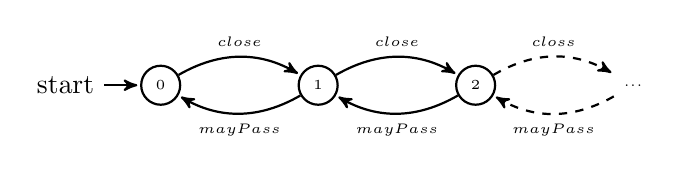
\begin{tikzpicture}[->,>=stealth',shorten >=1pt,auto,node distance=2cm,
  thick,main node/.style={circle,fill=white,draw,font=\sffamily\tiny\bfseries},
  sub node/.style={circle,fill=white,draw,font=\sffamily\tiny\bfseries},
  red node/.style={circle,fill=white,draw,font=\sffamily\tiny\bfseries},
  rec node/.style={rectangle,fill=white,draw,font=\sffamily\tiny\bfseries}]

  \node[initial,main node] (1) [] {$0$};
  \node[main node] (2) [right of=1] {$1$};
  \node[main node] (3) [right of=2]{$2$};
  \node[rec node,draw=none] (4) [right of=3]{$...$};

 	\path[every node/.style={font=\sffamily\tiny},dashed]
    (3) edge [bend left] node {$closs$} (4)
    (4) edge [bend left] node {$mayPass$} (3)
    ;

    \path[every node/.style={font=\sffamily\tiny}]
    (1) edge [bend left] node {$close$} (2)
    (2) edge [bend left] node {$close$} (3)
    (3) edge [bend left] node {$mayPass$} (2)
    (2) edge [bend left] node {$mayPass$} (1)
    ;

\end{tikzpicture}
\caption{The automata of $c_{close} \prec c_{mayPass}$}
\label{prop1_1}
\end{figure}

\begin{figure}[htp]
\centering
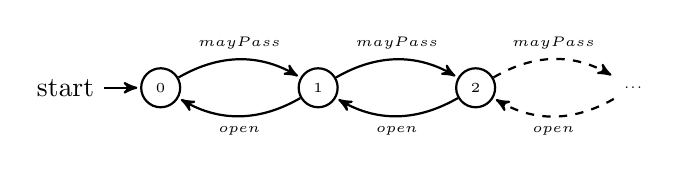
\begin{tikzpicture}[->,>=stealth',shorten >=1pt,auto,node distance=2cm,
  thick,main node/.style={circle,fill=white,draw,font=\sffamily\tiny\bfseries},
  sub node/.style={circle,fill=white,draw,font=\sffamily\tiny\bfseries},
  red node/.style={circle,fill=white,draw,font=\sffamily\tiny\bfseries},
  rec node/.style={rectangle,fill=white,draw,font=\sffamily\tiny\bfseries}]

  \node[initial,main node] (1) [] {$0$};
  \node[main node] (2) [right of=1] {$1$};
  \node[main node] (3) [right of=2]{$2$};
  \node[rec node,draw=none] (4) [right of=3]{$...$};

 	\path[every node/.style={font=\sffamily\tiny},dashed]
    (3) edge [bend left] node {$mayPass$} (4)
    (4) edge [bend left] node {$open$} (3)
    ;

    \path[every node/.style={font=\sffamily\tiny}]
    (1) edge [bend left] node {$mayPass$} (2)
    (2) edge [bend left] node {$mayPass$} (3)
    (3) edge [bend left] node {$open$} (2)
    (2) edge [bend left] node {$open$} (1)
    ;

\end{tikzpicture}
\caption{The automata of $c_{mayPass} \prec c_{open}$}
\label{prop1_2}
\end{figure}

\begin{figure}[htp]
\centering
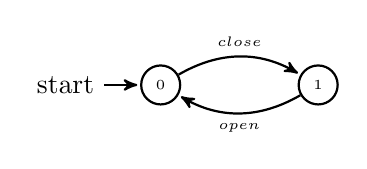
\begin{tikzpicture}[->,>=stealth',shorten >=1pt,auto,node distance=2cm,
  thick,main node/.style={circle,fill=white,draw,font=\sffamily\tiny\bfseries},
  sub node/.style={circle,fill=white,draw,font=\sffamily\tiny\bfseries},
  red node/.style={circle,fill=white,draw,font=\sffamily\tiny\bfseries},
  rec node/.style={rectangle,fill=white,draw,font=\sffamily\tiny\bfseries}]

  \node[initial,main node] (1) [] {$0$};
  \node[main node] (2) [right of=1] {$1$};

 	\path[every node/.style={font=\sffamily\tiny},dashed]
    ;

    \path[every node/.style={font=\sffamily\tiny}]
    (1) edge [bend left] node {$close$} (2)
    (2) edge [bend left] node {$open$} (1)
    ;

\end{tikzpicture}
\caption{The automata of $c_{close}$ \textbf{Alternate} $c_{open}$}
\label{prop1_3}
\end{figure}

\begin{figure}[htp]
\centering
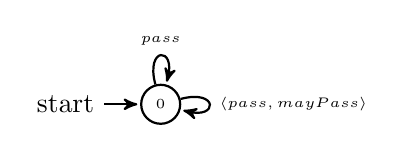
\begin{tikzpicture}[->,>=stealth',shorten >=1pt,auto,node distance=2cm,
  thick,main node/.style={circle,fill=white,draw,font=\sffamily\tiny\bfseries},
  sub node/.style={circle,fill=white,draw,font=\sffamily\tiny\bfseries},
  red node/.style={circle,fill=white,draw,font=\sffamily\tiny\bfseries},
  rec node/.style={rectangle,fill=white,draw,font=\sffamily\tiny\bfseries}]

  \node[initial,main node] (1) [] {$0$};

 	\path[every node/.style={font=\sffamily\tiny},dashed]
    ;

    \path[every node/.style={font=\sffamily\tiny}]
    (1) edge [loop above] node {$pass$} (1)
    (1) edge [loop right] node {$\langle pass,mayPass\rangle$} (1)
    ;

\end{tikzpicture}
\caption{The automata of $c_{close}$ \textbf{Alternate} $c_{open}$}
\label{prop1_4}
\end{figure}

\begin{figure}[htp]
\centering
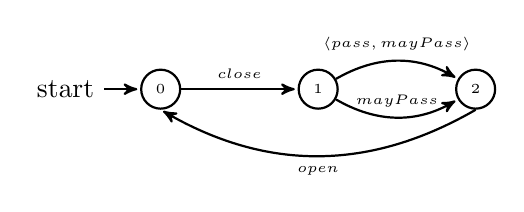
\begin{tikzpicture}[->,>=stealth',shorten >=1pt,auto,node distance=2cm,
  thick,main node/.style={circle,fill=white,draw,font=\sffamily\tiny\bfseries},
  sub node/.style={circle,fill=white,draw,font=\sffamily\tiny\bfseries},
  red node/.style={circle,fill=white,draw,font=\sffamily\tiny\bfseries},
  rec node/.style={rectangle,fill=white,draw,font=\sffamily\tiny\bfseries}]

  \node[initial,main node] (1) [] {$0$};
  \node[main node] (2) [right of=1] {$1$};
  \node[main node] (3) [right of=2] {$2$};

 	\path[every node/.style={font=\sffamily\tiny},dashed]
    ;

    \path[every node/.style={font=\sffamily\tiny}]
    (1) edge node {$close$} (2)
    (2) edge [bend left] node {$\langle pass,mayPass\rangle$} (3)
    (2) edge [bend right] node {$mayPass$} (3)
    (3.south) edge [bend left] node {$open$} (1.south)
    ;

\end{tikzpicture}
\caption{The automata of \textbf{Property 1}}
\label{prop1_ta}
\end{figure}

In practice, we convert \textbf{Property 1} into UPPAAL TA, which is shown in Fig.~\ref{uppaal_prop1}.
In the UPPAAL TA of \textbf{Property 1}, we define each event as 'channels', in order to synchronize with the Train and Gate system. We also change the corresponding actions in Train and Gate system into the right channels. Fig.~\ref{3sys} in Appendix A shows a possible running state diagram of system where three agents run concurrently. Note that in the UPPAAL TA of \textbf{Property 1} (Fig.~\ref{uppaal_prop1}), we omit the event 'mayPass' since no such action exists in Train system.

\begin{figure}[htp]
\centering
\includegraphics[width=2.5in]{graph/CCSL_prop1.png}
\caption{The UPPAAL TA of \textbf{Property 1}}
\label{uppaal_prop1}
\end{figure}

In UPPAAL, the nested statement with $\bff{AG}$ and $\bff{EF}$ is not allowed for some reasons. That means that we can not proof the liveness of CCSL clock by using the CTL statement '$\bff{AG} (\bff{EF} s)$'. Since the TA of \textbf{Property 1} in our example is a 'circle', so in fact we only need to guarantee the satisfaction of one of states, and thus other states's liveness is guaranteed. On the other side, not checking the liveness of CCSL clock alone, we instead check the occurrence of clock '$c_{close}$' each time after Gate is 'closed'. So we check the liveness of CCSL clock in our example by the following CTL statement on UPPAAL:

\begin{center}
    $\bff{AG} (gate\_close \rightarrow (\bff{AF}\ pass\_ticks))$,
\end{center}

$\bff{AF}$ is the operator in CTL. The CTL statement means that whenever gate is closed, the clock '$c_{pass}$' will eventually tick. UPPAAL supports this expression. Fig.~\ref{veriprop1} in Appendix A shows a result of the verification of \textbf{Property 1}.

The TA of \textbf{Property 2} is more complex since it contains time issues. It consists of 4 atomic CCSL expressions:

\begin{center}
\begin{enumerate}[1.]
    \item $c_{appr} \prec c_{close}$
    \item $c_{close} \prec c_{appr\_delay}$
    \item $c_{appr\_delay} = c_{appr}$ \textbf{delay} $1000$ \textbf{on} $c_{time}$
    \item $c_{time} =$ \textbf{IdealClock} \textbf{DiscretizeBy} $1$ ms
\end{enumerate}
\end{center}

In \cite{andre08}, how to encode the expressions with '\textbf{delay on}', '\textbf{DiscretizeBy}' and '\textbf{IdealClock}' into TA is illustrated in detail. Here we only give the transformed TAs. Fig.~\ref{prop2_3}, Fig.~\ref{prop2_4} shows the corresponding TA of expression 3 and 4 given above. Fig.~\ref{prop2} gives the TA of \textbf{Property 2}. The TAs of expression 1 and 2 are similar to Fig.~\ref{prop1_1} and Fig.~\ref{prop1_2}, which are omitted here.

\begin{figure}[htp]
\centering
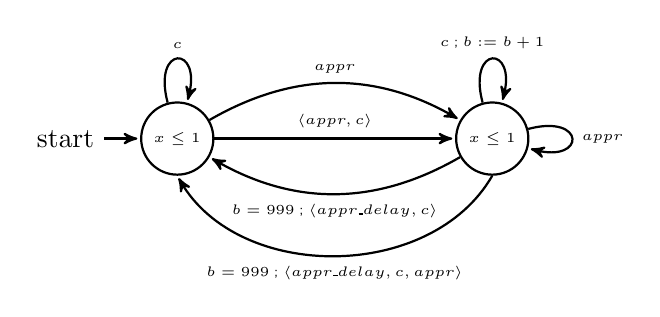
\begin{tikzpicture}[->,>=stealth',shorten >=1pt,auto,node distance=4cm,
  thick,main node/.style={circle,fill=white,draw,font=\sffamily\tiny\bfseries},
  sub node/.style={circle,fill=white,draw,font=\sffamily\tiny\bfseries},
  red node/.style={circle,fill=white,draw,font=\sffamily\tiny\bfseries},
  rec node/.style={rectangle,fill=white,draw,font=\sffamily\tiny\bfseries}]

  \node[initial,main node] (1) [] {$x\le 1$};
  \node[main node] (2) [right of=1] {$x\le 1$};

 	\path[every node/.style={font=\sffamily\tiny},dashed]
    ;

    \path[every node/.style={font=\sffamily\tiny}]
    (1) edge [bend left] node {$appr$} (2)
    (1) edge node {$\langle appr,c\rangle$} (2)
    (2) edge [bend left] node {$b=999$ ; $\langle appr\_delay, c\rangle$} (1)
    (2.south) edge [bend left=60] node {$b=999$ ; $\langle appr\_delay, c, appr\rangle$} (1.south)
    (1) edge [loop above] node {$c$} (1)
    (2) edge [loop above] node {$c$ ; $b:=b+1$} (2)
    (2) edge [loop right] node {$appr$} (2)
    ;

\end{tikzpicture}
\caption{The TA of $c_{appr\_delay} = c_{appr}$ \textbf{delay} $1000$ \textbf{on} $c_{time}$}
\label{prop2_3}
\end{figure}

\begin{figure}[htp]
\centering
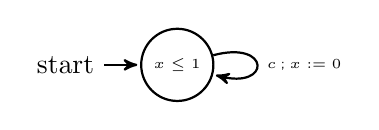
\begin{tikzpicture}[->,>=stealth',shorten >=1pt,auto,node distance=4cm,
  thick,main node/.style={circle,fill=white,draw,font=\sffamily\tiny\bfseries},
  sub node/.style={circle,fill=white,draw,font=\sffamily\tiny\bfseries},
  red node/.style={circle,fill=white,draw,font=\sffamily\tiny\bfseries},
  rec node/.style={rectangle,fill=white,draw,font=\sffamily\tiny\bfseries}]

  \node[initial,main node] (1) [] {$x\le 1$};

 	\path[every node/.style={font=\sffamily\tiny},dashed]
    ;

    \path[every node/.style={font=\sffamily\tiny}]
    (1) edge [loop right] node {$c$ ; $x:=0$} (1)

    ;

\end{tikzpicture}
\caption{The TA of $c_{time} =$ \textbf{IdealClock} \textbf{DiscretizeBy} $1$ ms}
\label{prop2_4}
\end{figure}

\begin{figure}[htp]
\centering
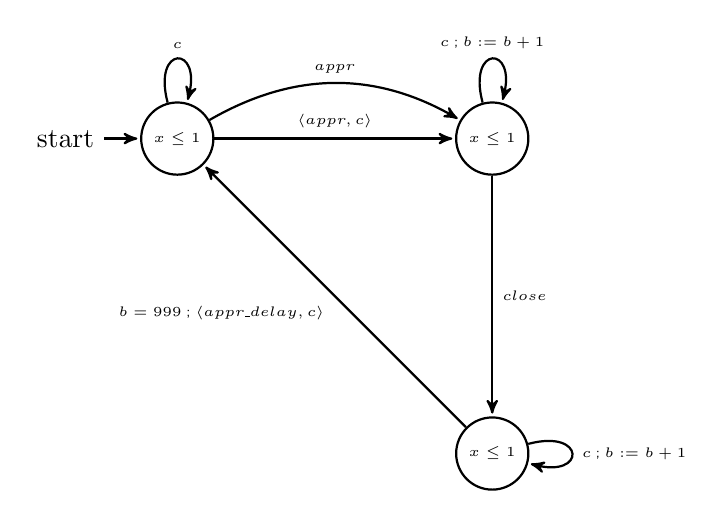
\begin{tikzpicture}[->,>=stealth',shorten >=1pt,auto,node distance=4cm,
  thick,main node/.style={circle,fill=white,draw,font=\sffamily\tiny\bfseries},
  sub node/.style={circle,fill=white,draw,font=\sffamily\tiny\bfseries},
  red node/.style={circle,fill=white,draw,font=\sffamily\tiny\bfseries},
  rec node/.style={rectangle,fill=white,draw,font=\sffamily\tiny\bfseries}]

  \node[initial,main node] (1) [] {$x\le 1$};
  \node[main node] (2) [right of=1] {$x\le 1$};
    \node[main node] (3) [below of=2] {$x\le 1$};

 	\path[every node/.style={font=\sffamily\tiny},dashed]
    ;

    \path[every node/.style={font=\sffamily\tiny}]
    (1) edge [bend left] node {$appr$} (2)
    (1) edge node {$\langle appr,c\rangle$} (2)
    (3) edge node {$b=999$ ; $\langle appr\_delay, c\rangle$} (1)
    %(3) edge [bend left] node {$b=999$ ; $\langle appr\_delay, c, appr\rangle$} (1.south)
    (1) edge [loop above] node {$c$} (1)
    (2) edge [loop above] node {$c$ ; $b:=b+1$} (2)
    (3) edge [loop right] node {$c$ ; $b:=b+1$} (3)
    (2) edge node {$close$} (3)
    %(2) edge [loop right] node {$appr$} (2)
    ;

\end{tikzpicture}
\caption{The TA of \textbf{Property 2}}
\label{prop2}
\end{figure}

In practice, we encoded \textbf{Property 2} into UPPAAL TA. Fig.~\ref{uppaal_prop2} shows its corresponding UPPAAL TA. We choose the CTL expression as follows for the same reason as for \textbf{Property 1}:

\begin{center}
    \textbf{AG} $(train\_appr \rightarrow$ \textbf{AF} $(close\_ticks))$
\end{center}

It means that whenever train approaches, the clock '$c_{close}$' will eventually tick.

We omit the result of verification of \textbf{Property 2}.

\begin{figure}[htp]
\centering
\includegraphics[width=2.5in]{graph/CCSL_prop2.png}
\caption{The UPPAAL TA of \textbf{Property 2}}
\label{uppaal_prop2}
\end{figure}

\section{Conclusion}
In this paper, we proposed a verification framework where we use STeC as a formal modeling language and CCSL as a specification language based on Timed Automatas. We mainly focus on the definition of CCSL in the domain of STeC and the encoding from STeC into TA. We also implement an automatic tool for such transformation and apply UPPAAL as a verification tool to our STeC-models in practice. At last we give a simple example of ITS system to illustrate how to put our proposed verification framework into work both in theory and practice.

As for the future work, in this paper, we give the encoding from STeC to TA, but the equivalence between STeC formula and translated TA has not yet been proofed.
\ifx
And we also will focus on the implementation of new a verification platform that based on our proposed verification framework where using STeC and CCSL as formal methods, even though . By now we only have an automatic tool for the encoding from STeC into TA. But for CCSL, such a tool demands to be built.
\fi


% conference papers do not normally have an appendix


% use section* for acknowledgement
\section*{Acknowledgment}
This work is supported by the INRIA
Associated Team DAESD between INRIA and ECNU, NSFC (No.
61021004 and No. 61370100) and Shanghai Knowledge Service Platform
Project (No. ZF1213).




% trigger a \newpage just before the given reference
% number - used to balance the columns on the last page
% adjust value as needed - may need to be readjusted if
% the document is modified later
%\IEEEtriggeratref{8}
% The "triggered" command can be changed if desired:
%\IEEEtriggercmd{\enlargethispage{-5in}}

% references section

% can use a bibliography generated by BibTeX as a .bbl file
% BibTeX documentation can be easily obtained at:
% http://www.ctan.org/tex-archive/biblio/bibtex/contrib/doc/
% The IEEEtran BibTeX style support page is at:
% http://www.michaelshell.org/tex/ieeetran/bibtex/
%\bibliographystyle{IEEEtran}
% argument is your BibTeX string definitions and bibliography database(s)
%\bibliography{IEEEabrv,../bib/paper}
%
% <OR> manually copy in the resultant .bbl file
% set second argument of \begin to the number of references
% (used to reserve space for the reference number labels box)
%~\cite{Ouaknine_timedcsp}

\bibliographystyle{ieeetr}
\bibliography{ref}{}


\ifx
\begin{thebibliography}{1}

\bibitem{hoare78}C.A.R Hoare.
  \emph{Communicating Sequential Processes}.
  Communications of ACM,
  Volume 21 No. 8,
  1978.

\bibitem{schneider06}Joel Ouaknine,Steve Schneider.
\emph{Timed CSP:A Retrospective}.
Electronic Notes in Theoretical Computer
Science,
162 (2006) 273C276.

\bibitem{milner86}Robin Milner.
\emph{A Calculus of Communicating Systems
}.
Computer Science,
Vol.92,
1986.

\bibitem{schneider95} Steve Schneider
.
\emph{An Operational Semantics for Timed CSP
}.
Information and Computation,
116:193-213,
1995.

\bibitem{alur94}R. Alur and D. L. Dill
.
  \emph{A theory of timed automata
}.
Theoretical Computer Science,
126(2):183-235,
1994.

\bibitem{chen10}Yixiang Chen.
\emph{STeC: A Location-Triggered Specification Language For Real-Time Systems}.
Science
China,
Vol.53,
No.1-18, 2010.

\bibitem{mallet08}Charles Andre, Frederic Mallet.
\emph{Clock Constraints in UML/MARTE CCSL}.
Research Report of
Research Unit of INRIA Sophia Antipolis,
2008.

\bibitem{mallet11}Regis Gascon, Frederic Mallet, Julien DeAntoni.
\emph{Logical time and temporal logics: comparing UML MARTE/CCSL and PSL}.
Temporal Representation and Reasoning (TIME),
pp 141-148,
2011.

\bibitem{mallet1302}Frederic Mallet, Jean-Vivien Millo, Yuliia Romenska.
\emph{State-based
representation of CCSL
operators}.
Research Report of Project-Team Aoste of INRIA Sophia Antipolis,
2013.

\bibitem{mallet13}Jagadish Suryadevara, Cristina Seceleanu, Frederic Mallet and Paul Pettersson.
\emph{Verifying MARTE/CCSL Mode Behaviors using
UPPAAL}.
11th International Conference on Software Engineering and Formal Methods,
Volume 8137,
pp 1-15,
2013.

\bibitem{andre09}Charles Andre.
\emph{Syntax and Semantics of the Clock Constraint Specification Language(CCSL)}.
Research Report of Research Unit of INRIA Sophia Antipolis,
2009.

\bibitem{cattani05}Stefano Cattani and Marta Kwiatkowska.
\emph{A Refinement-based Process Algebra
for Timed Automata}.
Under consideration for publication in Formal Aspects of Computing,
17(2),
pages 138-159,
Springer.
August 2005.

\bibitem{wangyi10}Parosh Aziz Abdulla, Pavek Krcal and Yi Wang.
\emph{Sampled semantics of times automata}.
Logical
Methods in Computer Science,
Vol. 6 (3:14): 1-37,
2010.

\bibitem{wu13}Hengyang Wu, Yixiang Chen and Min Zhang
\emph{On Denotational Semantics of Spatio-Temporal
Consistency Language STeC}.
International Symposium on Theoretical Aspects of Software Engineering,
pages 113-120,
2013.

\bibitem{mallet10}Frederic Mallet.
\emph{Logical Time in Model-Driven Engineering}.
University of Sophia Antipolis,
2010.

\bibitem{galyna}Iryna Zaretska, Galyna Zholtkevych, Grygoriy Zholtkevych.
\emph{Clocks Model for Specification and
Analysis of Timing in Real-Time Embedded Systems}.

\bibitem{OMG}OMG.
\emph{UML Profile for MARTE, v1.0}.
Object Management Group,
2009.

\bibitem{gastin08}Volker Diekert, Paul Gastin.
\emph{First-order definable languages}.
Logic and Automata: History and Perspectives, Texts in Logic and Games,
2008.

\bibitem{alur95}Rajeev Alur, David Dill.
\emph{Automata-theoretic Verification of Real-time Systems}.
1995.

\ifx
\bibitem{wangyi06}Elena Fersman, Leonid Mokrushin, Paul Pattersson, Wang Yi.
\emph{Schedulability analysis of fixed-priority
systems using timed automata}.
Theoretical Computer Science,
354: 301-317,
2006.

\fi

\ifx
\bibitem{roscoe01}G.M.Reed and A.W.Roscoe.
\emph{A timed model for communicating sequential processes}.
Theoretical
Computer Science,
58:249-261.

\bibitem{schneider9502}J.Davies,S.A.Schneider.
\emph{A brief history of times CSP}.
Theoretical Computer Science,
138(2):243-271,
1995.
\fi

\bibitem{roscoe}A.W.Roscoe.
\emph{A CSP solution to the "trains" problem}.
Programming Research Group,
University of Oxford.


\ifx
\bibitem{IEEEhowto:kopka}
H.~Kopka and P.~W. Daly, \emph{A Guide to \LaTeX}, 3rd~ed.\hskip 1em plus
  0.5em minus 0.4em\relax Harlow, England: Addison-Wesley, 1999.
\fi
\end{thebibliography}
\fi

\appendices
\section{Additional Figures About UPPAAL Verification}
\begin{figure*}[htp]
\centering
\includegraphics[scale=0.5]{graph/Train_TA_uppaal.png}
\caption{The Uppaal TA of Train Agent From 'STeC Code'}
\label{uppaalta}
\end{figure*}

\begin{figure*}[htp]
\centering
\includegraphics[scale=0.5]{graph/Gate_TA_uppaal.png}
\caption{The Uppaal TA of Gate Agent From 'STeC Code'}
\label{uppaalta2}
\end{figure*}

\begin{figure*}[htp]
\centering
\includegraphics[scale=0.5]{graph/running.png}
\caption{The running state diagram of $A_{Sys}$ for \textbf{Property 1}}
\label{3sys}
\end{figure*}

\begin{figure}[htp]
\centering
\includegraphics[width=2.5in]{graph/veri.jpg}
\caption{The result of verification of \textbf{Property 1}}
\label{veriprop1}
\end{figure}
% that's all folks
\end{document}




